\section{Sequential Chips}

  Now that we know how the NAND gate---and therefore every other fundamental gate---works, and we have constructed the clock, the next natural step is to be able to store a string of bits.\footnote{Most courses teach combinational logic first and then sequential, but this may not be the most optimal dependency sequence for two reasons. We can indeed do arithmetic without memory by directly applying an electric current to the input wires in a circuit, but this severely limits the computation that we can do. We would essentially have to do everything in ``one shot'' and immediately collect the results. While this is fine for addition, I cannot introduce an efficient schema of multiplication without knowing how to bit-shift, which is dependent on some form of memory. On a broader scale, almost all algorithms we worked with require some memory at some point, so memory may be more fundamental than computation. Thanks the Phillip Williams for talking with me on this!} Computers must be equipped with memory elements that can preserve data over time. These memory elements are built from \textit{sequential chips}. 

\subsection{SR Latches}

  Ideally, we would like a way to store a bit in memory, and this can be done by cross-coupling gates with each other, forming a sort of positive feedback.Therefore, given a certain signal into our circuit which we call a \textit{latch}, the outputs remain locked---or ``latched''---into a state. 

  \begin{definition}[SR Latch]
    The \textbf{set-reset (SR) latch} is a circuit that stores 1-bit memory. This is based on \textit{pulses} and we do not care about the duration of a signal. That is, if we activate a signal to inputs $S, R$ at \textit{any} point in time, then the output $Q$ will remain locked in some state, even \textit{after} the input signal disappears. 
  \end{definition}

  The SR latch---like all electronic circuits---require power to work, labeled with $S$ and $R$. The output is really just $Q$, but we can add redundancy by making the inverse $\overline{Q}$ available as well. There are two implementations of an SRlatch, which have symmetric behaviors. 

  \begin{theorem}[Active High SR Latch]
    A NOR SR latch can be implemented in the following circuit below, with its corresponding truth table. 

    \begin{figure}[H]
      \centering
      \begin{subfigure}[b]{0.48\textwidth}
        \centering
        \begin{tikzpicture}[circuit logic US]
          \node[nor gate] (nor1) at (0, 1) {}; 
          \node[nor gate] (nor2) at (0, -1) {}; 

          \node[left] at (-1.5, 1.1) {$S$}; 
          \node[left] at (-1.5, -1.1) {$R$}; 
          \node[right] at (2, 1) {$Q$};
          \node[right] at (2, -1) {$\overline{Q}$};

          \draw (-1.5, 1.1) -| (nor1.input 1);
          \draw (-1.5, -1.1) -| (nor2.input 2);
          \draw (nor1.output) |- (2, 1); 
          \draw (nor2.output) |- (2, -1); 

          \draw (nor1.output) |- (1.5, 1) -- (1.5, 0.8) -- (-1, -0.7) -- (-1, -0.9) |- (nor2.input 1);
          \draw (nor2.output) |- (1.5, -1) -- (1.5, -0.8) -- (-1, 0.7) -- (-1, 0.9) |- (nor1.input 2);
          \fill (1.5,1) circle (1.5pt);
          \fill (1.5,-1) circle (1.5pt);
        \end{tikzpicture} 
        \caption{Circuit diagram.}
      \end{subfigure}
      \hfill 
      \begin{subfigure}[b]{0.48\textwidth}
        \centering
        \begin{tabular}{|c|c|c|c|}
          \hline
          \textbf{S} & \textbf{R} & \textbf{Q} & \textbf{$\overline{Q}$} \\
          \hline
          0 & 0 & 1 & 0 \\
            &   & 0 & 1 \\
          \hline
          0 & 1 & 0 & 1 \\
          \hline
          1 & 0 & 1 & 0 \\
          \hline
          1 & 1 & 0 & 0 \\
          \hline
        \end{tabular} 
        \caption{Truth table.}
      \end{subfigure}
      \caption{XOR SR Latch. This is }
    \end{figure}

    Setting both $R = S = 1$ would result in an invalid state since they would attempt to turn $Q$ back and forth between $0$ and $1$, giving us a race condition. 

    \begin{figure}[H]
      \centering
      \begin{subfigure}[b]{0.48\textwidth}
        \centering
        \begin{tikzpicture}[circuit logic US]
          \node[nor gate] (nor1) at (0, 1) {}; 
          \node[nor gate] (nor2) at (0, -1) {}; 

          \node[left] at (-1.5, 1.1) {$S$}; 
          \node[left] at (-1.5, -1.1) {$R$}; 
          \node[right] at (2, 1) {$Q$};
          \node[right] at (2, -1) {$\overline{Q}$};

          \draw[blue] (-1.5, 1.1) -| (nor1.input 1);
          \draw[blue] (-1.5, -1.1) -| (nor2.input 2);
          \draw[red] (nor1.output) |- (2, 1); 
          \draw[blue] (nor2.output) |- (2, -1); 

          \draw[red] (nor1.output) |- (1.5, 1) -- (1.5, 0.8) -- (-1, -0.7) -- (-1, -0.9) |- (nor2.input 1);
          \draw[blue] (nor2.output) |- (1.5, -1) -- (1.5, -0.8) -- (-1, 0.7) -- (-1, 0.9) |- (nor1.input 2);
          \fill[red] (1.5,1) circle (1.5pt);
          \fill[blue] (1.5,-1) circle (1.5pt);
        \end{tikzpicture} 
        \caption{}
      \end{subfigure}
      \hfill 
      \begin{subfigure}[b]{0.48\textwidth}
        \centering
        \begin{tikzpicture}[circuit logic US]
          \node[nor gate] (nor1) at (0, 1) {}; 
          \node[nor gate] (nor2) at (0, -1) {}; 

          \node[left] at (-1.5, 1.1) {$S$}; 
          \node[left] at (-1.5, -1.1) {$R$}; 
          \node[right] at (2, 1) {$Q$};
          \node[right] at (2, -1) {$\overline{Q}$};

          \draw[blue] (-1.5, 1.1) -| (nor1.input 1);
          \draw[blue] (-1.5, -1.1) -| (nor2.input 2);
          \draw[blue] (nor1.output) |- (2, 1); 
          \draw[red] (nor2.output) |- (2, -1); 

          \draw[blue] (nor1.output) |- (1.5, 1) -- (1.5, 0.8) -- (-1, -0.7) -- (-1, -0.9) |- (nor2.input 1);
          \draw[red] (nor2.output) |- (1.5, -1) -- (1.5, -0.8) -- (-1, 0.7) -- (-1, 0.9) |- (nor1.input 2);
          \fill[blue] (1.5,1) circle (1.5pt);
          \fill[red] (1.5,-1) circle (1.5pt);
        \end{tikzpicture} 
        \caption{}
      \end{subfigure}
      \caption{Two possible initial states. The default state is $R = 0, S = 0$, which are both \textit{low states}, and $Q$ may be either $0$ or $1$. }
    \end{figure}

    If one of $R$ or $S$ is set to a high state, the latch is activated, and hence this is called an \textbf{active high SR latch}. Note that regardless of what the previous state the latch was in, the output signals are completely determined. 

    \begin{figure}[H]
      \centering
      \begin{subfigure}[b]{0.48\textwidth}
        \centering
        \begin{tikzpicture}[circuit logic US]
          \node[nor gate] (nor1) at (0, 1) {}; 
          \node[nor gate] (nor2) at (0, -1) {}; 

          \node[left] at (-1.5, 1.1) {$S$}; 
          \node[left] at (-1.5, -1.1) {$R$}; 
          \node[right] at (2, 1) {$Q$};
          \node[right] at (2, -1) {$\overline{Q}$};

          \draw[red] (-1.5, 1.1) -| (nor1.input 1);
          \draw[blue] (-1.5, -1.1) -| (nor2.input 2);
          \draw[blue] (nor1.output) |- (2, 1); 
          \draw[red] (nor2.output) |- (2, -1); 

          \draw[blue] (nor1.output) |- (1.5, 1) -- (1.5, 0.8) -- (-1, -0.7) -- (-1, -0.9) |- (nor2.input 1);
          \draw[red] (nor2.output) |- (1.5, -1) -- (1.5, -0.8) -- (-1, 0.7) -- (-1, 0.9) |- (nor1.input 2);
          \fill[blue] (1.5,1) circle (1.5pt);
          \fill[red] (1.5,-1) circle (1.5pt);
        \end{tikzpicture} 
        \caption{If we send a signal $R = 1$, then $Q = 0$, and even if we reset $R = 0$, $Q$ is still locked at $0$. }
      \end{subfigure}
      \hfill 
      \begin{subfigure}[b]{0.48\textwidth}
        \centering
        \begin{tikzpicture}[circuit logic US]
          \node[nor gate] (nor1) at (0, 1) {}; 
          \node[nor gate] (nor2) at (0, -1) {}; 

          \node[left] at (-1.5, 1.1) {$S$}; 
          \node[left] at (-1.5, -1.1) {$R$}; 
          \node[right] at (2, 1) {$Q$};
          \node[right] at (2, -1) {$\overline{Q}$};

          \draw[blue] (-1.5, 1.1) -| (nor1.input 1);
          \draw[red] (-1.5, -1.1) -| (nor2.input 2);
          \draw[red] (nor1.output) |- (2, 1); 
          \draw[blue] (nor2.output) |- (2, -1); 

          \draw[red] (nor1.output) |- (1.5, 1) -- (1.5, 0.8) -- (-1, -0.7) -- (-1, -0.9) |- (nor2.input 1);
          \draw[blue] (nor2.output) |- (1.5, -1) -- (1.5, -0.8) -- (-1, 0.7) -- (-1, 0.9) |- (nor1.input 2);
          \fill[red] (1.5,1) circle (1.5pt);
          \fill[blue] (1.5,-1) circle (1.5pt);
        \end{tikzpicture} 
        \caption{If we send a signal $S = 1$, then $Q = 1$, and even if reset $S = 0$, $Q$ is still locked at $1$. }
      \end{subfigure}
      \caption{}
    \end{figure}
  \end{theorem}

  Now unlike the active high latches which are activated when the current is $1$, active low latches are activated when the current is $0$. 

  \begin{theorem}[Active Low SR Latch]
    A NAND SR latch can be implemented in the following circuit below, with its corresponding truth table. 
    
    \begin{figure}[H]
      \centering
      \begin{subfigure}[b]{0.48\textwidth}
        \centering
        \begin{tikzpicture}[circuit logic US]
          \node[nand gate] (nor1) at (0, 1) {}; 
          \node[nand gate] (nor2) at (0, -1) {}; 
          \node[left] at (-1.5, 1.1) {$S$}; 
          \node[left] at (-1.5, -1.1) {$R$}; 
          \node[right] at (2, 1) {$Q$};
          \node[right] at (2, -1) {$\overline{Q}$};

          \draw (-1.5, 1.1) -| (nor1.input 1);
          \draw (-1.5, -1.1) -| (nor2.input 2);
          \draw (nor1.output) |- (2, 1); 
          \draw (nor2.output) |- (2, -1); 

          \draw (nor1.output) |- (1.5, 1) -- (1.5, 0.8) -- (-1, -0.7) -- (-1, -0.9) |- (nor2.input 1);
          \draw (nor2.output) |- (1.5, -1) -- (1.5, -0.8) -- (-1, 0.7) -- (-1, 0.9) |- (nor1.input 2);
          \fill (1.5,1) circle (1.5pt);
          \fill (1.5,-1) circle (1.5pt);
        \end{tikzpicture} 
        \caption{Circuit diagram.}
      \end{subfigure}
      \hfill 
      \begin{subfigure}[b]{0.48\textwidth}
        \centering
        \begin{tabular}{|c|c|c|c|}
          \hline
          \textbf{S} & \textbf{R} & \textbf{Q} & \textbf{$\overline{Q}$} \\
          \hline
          0 & 0 & 1 & 1 \\
          \hline
          0 & 1 & 1 & 0 \\
          \hline
          1 & 0 & 0 & 1 \\
          \hline
          1 & 1 & 0 & 1 \\
            &   & 1 & 0 \\
          \hline
        \end{tabular}
        \caption{Truth table.}
      \end{subfigure}
      \caption{NAND SR Latch}
    \end{figure}

    Setting both $R = S = 0$ would result in an invalid state since they would attempt to turn $Q$ back and forth between $0$ and $1$, giving us a race condition. 

    \begin{figure}[H]
      \centering
      \begin{subfigure}[b]{0.48\textwidth}
        \centering
        \begin{tikzpicture}[circuit logic US]
          \node[nand gate] (nor1) at (0, 1) {}; 
          \node[nand gate] (nor2) at (0, -1) {}; 
          \node[left] at (-1.5, 1.1) {$S$}; 
          \node[left] at (-1.5, -1.1) {$R$}; 
          \node[right] at (2, 1) {$Q$};
          \node[right] at (2, -1) {$\overline{Q}$};

          \draw[red] (-1.5, 1.1) -- (nor1.input 1);
          \draw[red] (-1.5, -1.1) -- (nor2.input 2);
          \draw[blue] (nor1.output) -- (2, 1); 
          \draw[red] (nor2.output) -- (2, -1); 

          \draw[blue] (nor1.output) -- (1.5, 1) -- (1.5, 0.8) -- (-1, -0.7) -- (-1, -0.9) -- (nor2.input 1);
          \draw[red] (nor2.output) -- (1.5, -1) -- (1.5, -0.8) -- (-1, 0.7) -- (-1, 0.9) -- (nor1.input 2);
          \fill[blue] (1.5,1) circle (1.5pt);
          \fill[red] (1.5,-1) circle (1.5pt);
        \end{tikzpicture} 
        \caption{}
      \end{subfigure}
      \hfill 
      \begin{subfigure}[b]{0.48\textwidth}
        \centering
        \begin{tikzpicture}[circuit logic US]
          \node[nand gate] (nor1) at (0, 1) {}; 
          \node[nand gate] (nor2) at (0, -1) {}; 
          \node[left] at (-1.5, 1.1) {$S$}; 
          \node[left] at (-1.5, -1.1) {$R$}; 
          \node[right] at (2, 1) {$Q$};
          \node[right] at (2, -1) {$\overline{Q}$};

          \draw[red] (-1.5, 1.1) -- (nor1.input 1);
          \draw[red] (-1.5, -1.1) -- (nor2.input 2);
          \draw[red] (nor1.output) -- (2, 1); 
          \draw[blue] (nor2.output) -- (2, -1); 

          \draw[red] (nor1.output) -- (1.5, 1) -- (1.5, 0.8) -- (-1, -0.7) -- (-1, -0.9) -- (nor2.input 1);
          \draw[blue] (nor2.output) -- (1.5, -1) -- (1.5, -0.8) -- (-1, 0.7) -- (-1, 0.9) -- (nor1.input 2);
          \fill[red] (1.5,1) circle (1.5pt);
          \fill[blue] (1.5,-1) circle (1.5pt);
        \end{tikzpicture} 
        \caption{}
      \end{subfigure}
      \caption{The default state is $R = 1, S = 1$, i.e. they are both \textit{high states}, and $Q$ may be either $0$ or $1$. This is known as an \textbf{active low SR latch}. }
    \end{figure}

    If one of $R$ or $S$ is set to a low state, the latch is activated, and hence this is called an \textbf{active low SR latch}. Note that regardless of what the previous state the latch was in, the output signals are completely determined. 

    \begin{figure}[H]
      \centering
      \begin{subfigure}[b]{0.48\textwidth}
        \centering
        \begin{tikzpicture}[circuit logic US]
          \node[nand gate] (nor1) at (0, 1) {}; 
          \node[nand gate] (nor2) at (0, -1) {}; 
          \node[left] at (-1.5, 1.1) {$S$}; 
          \node[left] at (-1.5, -1.1) {$R$}; 
          \node[right] at (2, 1) {$Q$};
          \node[right] at (2, -1) {$\overline{Q}$};

          \draw[blue] (-1.5, 1.1) -| (nor1.input 1);
          \draw[red] (-1.5, -1.1) -| (nor2.input 2);
          \draw[red] (nor1.output) |- (2, 1); 
          \draw[blue] (nor2.output) |- (2, -1); 

          \draw[red] (nor1.output) |- (1.5, 1) -- (1.5, 0.8) -- (-1, -0.7) -- (-1, -0.9) |- (nor2.input 1);
          \draw[blue] (nor2.output) |- (1.5, -1) -- (1.5, -0.8) -- (-1, 0.7) -- (-1, 0.9) |- (nor1.input 2);
          \fill[red] (1.5,1) circle (1.5pt);
          \fill[blue] (1.5,-1) circle (1.5pt);
        \end{tikzpicture} 
        \caption{}
      \end{subfigure}
      \hfill 
      \begin{subfigure}[b]{0.48\textwidth}
        \centering
        \begin{tikzpicture}[circuit logic US]
          \node[nand gate] (nor1) at (0, 1) {}; 
          \node[nand gate] (nor2) at (0, -1) {}; 
          \node[left] at (-1.5, 1.1) {$S$}; 
          \node[left] at (-1.5, -1.1) {$R$}; 
          \node[right] at (2, 1) {$Q$};
          \node[right] at (2, -1) {$\overline{Q}$};

          \draw[red] (-1.5, 1.1) -| (nor1.input 1);
          \draw[blue] (-1.5, -1.1) -| (nor2.input 2);
          \draw[blue] (nor1.output) |- (2, 1); 
          \draw[red] (nor2.output) |- (2, -1); 

          \draw[blue] (nor1.output) |- (1.5, 1) -- (1.5, 0.8) -- (-1, -0.7) -- (-1, -0.9) |- (nor2.input 1);
          \draw[red] (nor2.output) |- (1.5, -1) -- (1.5, -0.8) -- (-1, 0.7) -- (-1, 0.9) |- (nor1.input 2);
          \fill[blue] (1.5,1) circle (1.5pt);
          \fill[red] (1.5,-1) circle (1.5pt);
        \end{tikzpicture} 
        \caption{}
      \end{subfigure}
      \caption{If we send a signal $S = 0$, then $Q = 0$, and even if reset $S = 1$, $Q$ is still locked at $0$. }
    \end{figure}
  \end{theorem}

  These signals may be noisy, and we might want more control over whether a latch can change states, i.e its \textit{transparency}. This is done by adding an extra \textit{gate} that explicitly tells us when the latch can change states. 

  \begin{definition}[Gated SR Latch]
    A \textbf{gated SR latch} is an SR latch that can only change state when it is enabled. This enabling is done with an additional 2 NAND gates, and so the SR latch is enabled only when $E = 1$. 

    \begin{figure}[H]
      \centering
      \begin{subfigure}[b]{0.48\textwidth}
        \centering
        \begin{tikzpicture}[circuit logic US]
          \node[nand gate] (nand1) at (-2, 1.1) {};
          \node[nand gate] (nand2) at (-2, -1.1) {};
          \node[nor gate] (nor1) at (0, 1) {}; 
          \node[nor gate] (nor2) at (0, -1) {}; 

          \draw (-3, 1.2) -- (nand1.input 1);
          \draw (-3, -1.2) -- (nand2.input 2);
          \draw (-3, 0) -- (-2.7, 0) -- (-2.7,1) -- (nand1.input 2);
          \draw (-3, 0) -- (-2.7, 0) -- (-2.7,-1) -- (nand2.input 1);
          \node[left] at (-3,0) {$E$};
          \node[left] at (-3,1.2) {$S$};
          \node[left] at (-3,-1.2) {$R$};
          \node[right] at (2, 1) {$Q$};
          \node[right] at (2, -1) {$\overline{Q}$};

          \draw (nand1.output) -- (nor1.input 1);
          \draw (nand2.output) -- (nor2.input 2);
          \draw (nor1.output) -- (2, 1); 
          \draw (nor2.output) -- (2, -1); 

          \draw (nor1.output) -- (1.5, 1) -- (1.5, 0.8) -- (-1, -0.7) -- (-1, -0.9) -- (nor2.input 1);
          \draw (nor2.output) -- (1.5, -1) -- (1.5, -0.8) -- (-1, 0.7) -- (-1, 0.9) -- (nor1.input 2);
          \fill (1.5,1) circle (1.5pt);
          \fill (1.5,-1) circle (1.5pt);
          \fill (-2.7,0) circle (1.5pt);
        \end{tikzpicture} 
        \caption{Gated XOR SR Latch.}
      \end{subfigure}
      \hfill 
      \begin{subfigure}[b]{0.48\textwidth}
        \centering
        \begin{tikzpicture}[circuit logic US]
          \node[nand gate] (nand1) at (-2, 1.1) {};
          \node[nand gate] (nand2) at (-2, -1.1) {};
          \node[nand gate] (nor1) at (0, 1) {}; 
          \node[nand gate] (nor2) at (0, -1) {}; 

          \draw (-3, 1.2) -- (nand1.input 1);
          \draw (-3, -1.2) -- (nand2.input 2);
          \draw (-3, 0) -- (-2.7, 0) -- (-2.7,1) -- (nand1.input 2);
          \draw (-3, 0) -- (-2.7, 0) -- (-2.7,-1) -- (nand2.input 1);
          \node[left] at (-3,0) {$E$};
          \node[left] at (-3,1.2) {$S$};
          \node[left] at (-3,-1.2) {$R$};
          \node[right] at (2, 1) {$Q$};
          \node[right] at (2, -1) {$\overline{Q}$};

          \draw (nand1.output) -- (nor1.input 1);
          \draw (nand2.output) -- (nor2.input 2);
          \draw (nor1.output) -- (2, 1); 
          \draw (nor2.output) -- (2, -1); 

          \draw (nor1.output) -- (1.5, 1) -- (1.5, 0.8) -- (-1, -0.7) -- (-1, -0.9) -- (nor2.input 1);
          \draw (nor2.output) -- (1.5, -1) -- (1.5, -0.8) -- (-1, 0.7) -- (-1, 0.9) -- (nor1.input 2);
          \fill (1.5,1) circle (1.5pt);
          \fill (1.5,-1) circle (1.5pt);
          \fill (-2.7,0) circle (1.5pt);
        \end{tikzpicture} 
        \caption{Gated NAND SR Latch.}
      \end{subfigure}
      \caption{Note that if $E = 0$, then the output of the leftmost two NAND gates will be $1$ no matter what, and so the values of $R, S$ does not have any effect. }
    \end{figure}
  \end{definition}

  \begin{example}[Active High Gated SR Latch]
    By keeping track of the voltages in the wires of interest and running them across a common time axis, we can visualize this circuit in action. Note that in here, we assume that electric current is instantaneous, resulting in the familiar \textit{square waves}. Let's look at an active high SR latch. 

    \begin{figure}[H]
      \centering 
      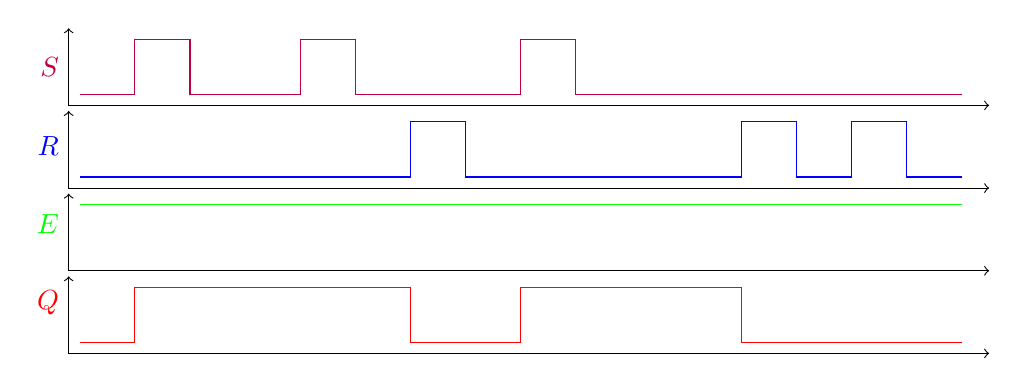
\begin{tikzpicture}[scale=0.7]
        \def\h{1.5}
        \draw[<->] (-0.2, 1.2) -- (-0.2, -0.2) -- (16.5, -0.2); 
        \draw[<->, yshift=-1.5cm] (-0.2, 1.2) -- (-0.2, -0.2) -- (16.5, -0.2); 
        \draw[<->, yshift=-3cm] (-0.2, 1.2) -- (-0.2, -0.2) -- (16.5, -0.2); 
        \draw[<->, yshift=-4.5cm] (-0.2, 1.2) -- (-0.2, -0.2) -- (16.5, -0.2); 
        \node[purple, left] at (-0.2, 0.5) {$S$}; 
        \node[blue, left, yshift=-1cm] at (-0.2, 0.5) {$R$}; 
        \node[green, left, yshift=-2cm] at (-0.2, 0.5) {$E$}; 
        \node[red, left, yshift=-3cm] at (-0.2, 0.5) {$Q$}; 

        \draw[purple] (0, 0) -- (1, 0) -- (1, 1) -- (2, 1) -- (2, 0) -- (4, 0) -- (4, 1) -- (5, 1) -- (5, 0) -- (8, 0) -- (8, 1) -- (9, 1) -- (9, 0) -- (16, 0);
        \draw[blue, yshift=-1.5cm] (0, 0) -- (6, 0) -- (6, 1) -- (7, 1) -- (7, 0) -- (12, 0) -- (12, 1) -- (13, 1) -- (13, 0) -- (14, 0) -- (14, 1) -- (15, 1) -- (15, 0) -- (16, 0);
        \draw[green, yshift=-3cm] (0, 1) -- (16, 1);
        \draw[red, yshift=-4.5cm] (0, 0) -- (1, 0) -- (1, 1) -- (6, 1) -- (6, 0) -- (8, 0) -- (8, 1) -- (12, 1) -- (12, 0) -- (16, 0);
      \end{tikzpicture}
      \caption{In here the gate is always enabled as $E = 1$ always. In the beginning $S = 1$ causing $Q = 1$, and this does not change until $R = 1$, at which point $Q = 0$. Note that the second pulse of $S$ does not affect the state because it is already $Q = 1$. Soon after $S = 1$ again, causing $Q = 1$ and when $R = 1$ $Q = 0$.}
    \end{figure}

    \begin{figure}[H]
      \centering 
      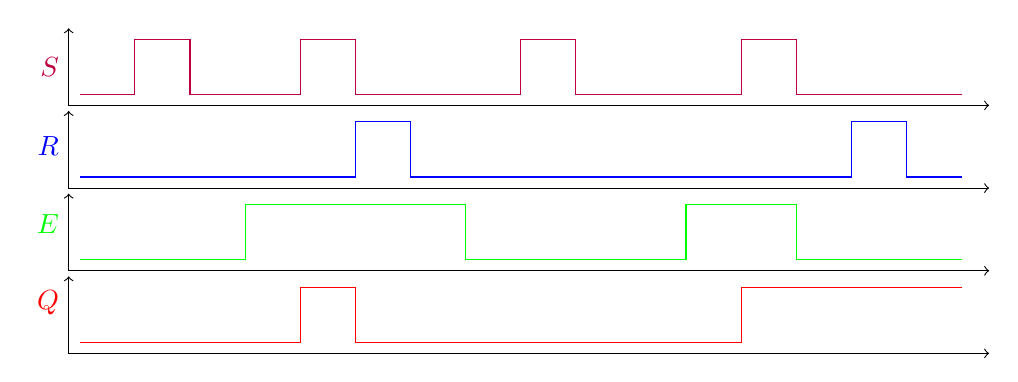
\begin{tikzpicture}[scale=0.7]
        \draw[<->] (-0.2, 1.2) -- (-0.2, -0.2) -- (16.5, -0.2); 
        \draw[<->, yshift=-1.5cm] (-0.2, 1.2) -- (-0.2, -0.2) -- (16.5, -0.2); 
        \draw[<->, yshift=-3cm] (-0.2, 1.2) -- (-0.2, -0.2) -- (16.5, -0.2); 
        \draw[<->, yshift=-4.5cm] (-0.2, 1.2) -- (-0.2, -0.2) -- (16.5, -0.2); 
        \node[purple, left] at (-0.2, 0.5) {$S$}; 
        \node[blue, left, yshift=-1cm] at (-0.2, 0.5) {$R$}; 
        \node[green, left, yshift=-2cm] at (-0.2, 0.5) {$E$}; 
        \node[red, left, yshift=-3cm] at (-0.2, 0.5) {$Q$}; 

        \draw[purple] (0, 0) -- 
          (1, 0) -- (1, 1) -- (2, 1) -- (2, 0) -- 
          (4, 0) -- (4, 1) -- (5, 1) -- (5, 0) -- 
          (8, 0) -- (8, 1) -- (9, 1) -- (9, 0) -- 
          (12, 0) -- (12, 1) -- (13, 1) -- (13, 0) -- 
          (16, 0);
        \draw[blue, yshift=-1.5cm] (0, 0) -- 
          (5, 0) -- (5, 1) -- (6, 1) -- (6, 0) -- 
          (14, 0) -- (14, 1) -- (15, 1) -- (15, 0) -- 
          (16, 0);
        \draw[green, yshift=-3cm] (0, 0) -- 
          (3, 0) -- (3, 1) -- (7, 1) -- (7, 0) -- 
          (11, 0) -- (11, 1) -- (13, 1) -- (13, 0) -- 
          (16, 0);
        \draw[red, yshift=-4.5cm] (0, 0) -- 
          (4, 0) -- (4, 1) -- (5, 1) -- (5, 0) -- 
          (12, 0) -- (12, 1) -- (16, 1);
      \end{tikzpicture}
      \caption{Now we toggle $E$ on and off throughout. We can start off by filling in all the places where $E = 1$, where we want $Q$ to basically copy $S$. At every other place, we just continue what the state $Q$ was in. } 
    \end{figure}
  \end{example}

\subsection{Level and Edge Triggered D-Latches}

  Note that we still have the problem of invalid signals. For example, if there was an instance that at the same clock time a signal of $S=1, R=1$ (on either an ungated latch or a gated latch with $E=1$), then both $Q$ and $\overline{Q}$ will be $1$, which will cause both to be $0$, and then $1$, and so on. This causes a race condition, which leads to unpredictable behavior. 

  \begin{figure}[H]
    \centering 
    \begin{tikzpicture}[circuit logic US]
      \node[nand gate] (nand1) at (-2, 1.1) {};
      \node[nand gate] (nand2) at (-2, -1.1) {};
      \node[nor gate] (nor1) at (0, 1) {}; 
      \node[nor gate] (nor2) at (0, -1) {}; 
      \node[not gate, point down, scale=0.8] (not1) at (-3.5, 0.8) {};

      \draw (-4, 1.2) -- (nand1.input 1);
      \draw (-4, 1.2) -- (-3.5, 1.2) -- (not1.input); 
      \draw (not1.output) -- (-3.5, 0.1) -- (-3.4, 0) -- (-3.5, -0.1) -- (-3.5, -1.2) -- (nand2.input 2);
      \draw (-4, 0) -- (-2.7, 0) -- (-2.7,1) -- (nand1.input 2);
      \draw (-4, 0) -- (-2.7, 0) -- (-2.7,-1) -- (nand2.input 1);
      \node[left] at (-4,0) {$E$};
      \node[left] at (-4,1.2) {$D$};
      \node[right] at (2, 1) {$Q$};
      \node[right] at (2, -1) {$\overline{Q}$};

      \draw (nand1.output) -- (nor1.input 1);
      \draw (nand2.output) -- (nor2.input 2);
      \draw (nor1.output) -- (2, 1); 
      \draw (nor2.output) -- (2, -1); 

      \draw (nor1.output) -- (1.5, 1) -- (1.5, 0.8) -- (-1, -0.7) -- (-1, -0.9) -- (nor2.input 1);
      \draw (nor2.output) -- (1.5, -1) -- (1.5, -0.8) -- (-1, 0.7) -- (-1, 0.9) -- (nor1.input 2);
      \fill (1.5,1) circle (1.5pt);
      \fill (1.5,-1) circle (1.5pt);
      \fill (-2.7,0) circle (1.5pt);
    \end{tikzpicture} 
    \caption{} 
  \end{figure}

  It turns out that we can simplify this circuit, making it cheaper to produce while still behaving identically. This gives us the D-latch. 

  \begin{definition}[Level Triggered D-Latch]
    The \textbf{(gated) data latch (D-latch)}, also called a \textbf{clocked D-latch}, gives us more control over storing a 1-bit in memory. 

    \begin{figure}[H]
      \centering
      \begin{subfigure}[b]{0.48\textwidth}
        \centering
        \begin{tikzpicture}
          \node[latch, align=center] (latch) at (0,0) {D Latch};
          \draw (latch.pin 1) -- ++(-0.5,0) node[left] {D};
          \draw (latch.pin 3) -- ++(-0.5,0) node[left] {E};
          \draw (latch.pin 6) -- ++(0.5,0) node[right] {Q};
          \draw (latch.pin 4) -- ++(0.5,0) node[right] {$\overline{Q}$};
        \end{tikzpicture}
      \end{subfigure}
      \hfill 
      \begin{subfigure}[b]{0.48\textwidth}
        \centering
          \begin{tabular}{|c|c|c|c|}
            \hline
            $E$ & $D$ & $Q$ & $\overline{Q}$ \\
            \hline
            0 & 0 & $Q_{\mathrm{prev}}$ & $\overline{Q_{\mathrm{prev}}}$ \\
            \hline
            0 & 1 & $Q_{\mathrm{prev}}$ & $\overline{Q_{\mathrm{prev}}}$ \\
            \hline
            1 & 0 & 0 & 1 \\
            \hline
            1 & 1 & 1 & 0 \\
            \hline
          \end{tabular}
      \end{subfigure}
      \caption{Chip notation and truth table of a D latch. Note that when $E = 0$, the latch simply outputs the previously stored element $Q = Q_{\mathrm{prev}}$. }
    \end{figure}

    \begin{figure}[H]
      \centering
      \begin{subfigure}[b]{0.48\textwidth}
        \centering
        \begin{tikzpicture}[circuit logic US]
          \node[nand gate] (nand1) at (-2, 1.1) {};
          \node[nand gate] (nand2) at (-2, -1.1) {};
          \node[nor gate] (nor1) at (0, 1) {}; 
          \node[nor gate] (nor2) at (0, -1) {}; 

          \draw (-3.5, 1.2) -- (nand1.input 1);
          \draw (-3.5, -1.2) -- (nand2.input 2);
          \node[left] at (-3.5,-1.2) {$E$};
          \node[left] at (-3.5,1.2) {$R$};
          \node[right] at (2, 1) {$Q$};
          \node[right] at (2, -1) {$\overline{Q}$};

          \draw (-3.5, -1.2) -- (-3.2, -1.2) -- (-3.2, 1) -- (nand1.input 2);
          \fill (-3.2, -1.2) circle (1.5pt);
          \draw (nand1.output) -- (-1.2, 1.1) -- (-1.2, 0.9) -- (-2.7, -0.9) -- (-2.7, -1) -- (nand2.input 1);

          \draw (nand1.output) -- (nor1.input 1);
          \draw (nand2.output) -- (nor2.input 2);
          \draw (nor1.output) -- (2, 1); 
          \draw (nor2.output) -- (2, -1); 

          \draw (nor1.output) -- (1.5, 1) -- (1.5, 0.8) -- (-1, -0.7) -- (-1, -0.9) -- (nor2.input 1);
          \draw (nor2.output) -- (1.5, -1) -- (1.5, -0.8) -- (-1, 0.7) -- (-1, 0.9) -- (nor1.input 2);
          \fill (1.5,1) circle (1.5pt);
          \fill (1.5,-1) circle (1.5pt);
        \end{tikzpicture} 
        \caption{Gated XOR SR Latch.}
      \end{subfigure}
      \hfill 
      \begin{subfigure}[b]{0.48\textwidth}
        \centering
        \begin{tikzpicture}[circuit logic US]
          \node[nand gate] (nand1) at (-2, 1.1) {};
          \node[nand gate] (nand2) at (-2, -1.1) {};
          \node[nand gate] (nor1) at (0, 1) {}; 
          \node[nand gate] (nor2) at (0, -1) {}; 

          \draw (-3.5, 1.2) -- (nand1.input 1);
          \draw (-3.5, -1.2) -- (nand2.input 2);
          \node[left] at (-3.5,-1.2) {$E$};
          \node[left] at (-3.5,1.2) {$R$};
          \node[right] at (2, 1) {$Q$};
          \node[right] at (2, -1) {$\overline{Q}$};

          \draw (-3.5, -1.2) -- (-3.2, -1.2) -- (-3.2, 1) -- (nand1.input 2);
          \fill (-3.2, -1.2) circle (1.5pt);
          \draw (nand1.output) -- (-1.2, 1.1) -- (-1.2, 0.9) -- (-2.7, -0.9) -- (-2.7, -1) -- (nand2.input 1);

          \draw (nand1.output) -- (nor1.input 1);
          \draw (nand2.output) -- (nor2.input 2);
          \draw (nor1.output) -- (2, 1); 
          \draw (nor2.output) -- (2, -1); 

          \draw (nor1.output) -- (1.5, 1) -- (1.5, 0.8) -- (-1, -0.7) -- (-1, -0.9) -- (nor2.input 1);
          \draw (nor2.output) -- (1.5, -1) -- (1.5, -0.8) -- (-1, 0.7) -- (-1, 0.9) -- (nor1.input 2);
          \fill (1.5,1) circle (1.5pt);
          \fill (1.5,-1) circle (1.5pt);
        \end{tikzpicture} 
        \caption{Gated NAND SR Latch.}
      \end{subfigure}
      \caption{}
    \end{figure}
  \end{definition}

  \begin{example}[Level Triggered D-Latch]
    The essence of the behavior is the output follows the input while $E$ is enabled. 

    \begin{figure}[H]
      \centering 
      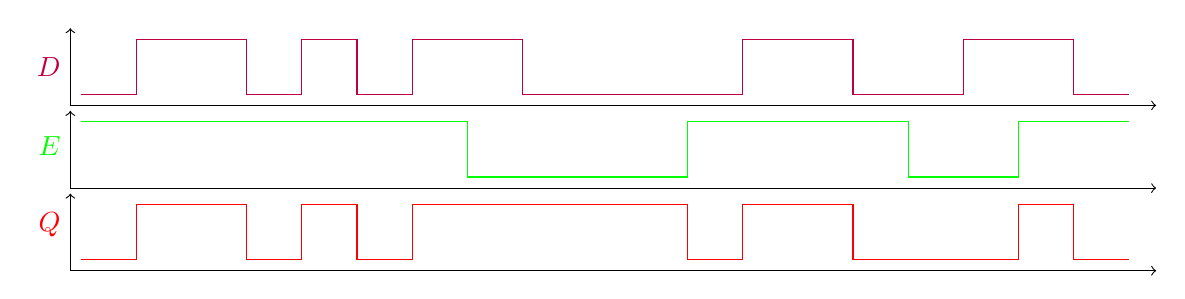
\begin{tikzpicture}[scale=0.7]
        \draw[<->] (-0.2, 1.2) -- (-0.2, -0.2) -- (19.5, -0.2); 
        \draw[<->, yshift=-1.5cm] (-0.2, 1.2) -- (-0.2, -0.2) -- (19.5, -0.2); 
        \draw[<->, yshift=-3cm] (-0.2, 1.2) -- (-0.2, -0.2) -- (19.5, -0.2); 
        \node[purple, left] at (-0.2, 0.5) {$D$}; 
        \node[green, left, yshift=-1cm] at (-0.2, 0.5) {$E$}; 
        \node[red, left, yshift=-2cm] at (-0.2, 0.5) {$Q$}; 

        \draw[purple] (0, 0) -- 
          (1, 0) -- (1, 1) -- (3, 1) -- (3, 0) -- 
          (4, 0) -- (4, 1) -- (5, 1) -- (5, 0) -- 
          (6, 0) -- (6, 1) -- (8, 1) -- (8, 0) -- 
          (12, 0) -- (12, 1) -- (14, 1) -- (14, 0) -- 
          (16, 0) -- (16, 1) -- (18, 1) -- (18, 0) -- 
          (19, 0);
        \draw[green, yshift=-1.5cm] 
          (0, 1) --  (7, 1) -- (7, 0) -- 
          (11, 0) -- (11, 1) -- (15, 1) -- (15, 0) -- 
          (17, 0) -- (17, 1) -- (19, 1);
        \draw[red, yshift=-3cm] (0, 0) -- 
          (1, 0) -- (1, 1) -- (3, 1) -- (3, 0) -- 
          (4, 0) -- (4, 1) -- (5, 1) -- (5, 0) -- 
          (6, 0) -- (6, 1) -- (11, 1) -- (11, 0) -- 
          (12, 0) -- (12, 1) -- (14, 1) -- (14, 0) -- 
          (17, 0) -- (17, 1) -- (18, 1) -- (18, 0) -- 
          (19, 0);
      \end{tikzpicture}
      \caption{Again, we just let the result $Q$ follow the input $D$ whenever $E = 1$,and continue the rest for when $E = 0$.}
    \end{figure}
  \end{example} 

  Therefore, if we want to store a bit of information, we set $E = 1$, collect that bit from $D$, and then set $E = 0$ to latch it in place. This behavior is quite stable for storing 1-bit, but we need more control when storing a multi-bit buffer, where we need several D-latches working in tandem. The general idea is that if we have a multi-bit buffer, we want a set of D-latches to be enabled and disabled at once. 

  \begin{figure}[H]
    \centering 
    \begin{tikzpicture}
      \foreach \h in {0, 2, 4} {
        \draw (0, 0+\h) rectangle (0.8, 1.2+\h);
        \draw (-3, 1+\h) -- (0, 1+\h); 
        \draw (0.8, 0.65+\h) -- (2, 0.65+\h); 
        \node[right, font=\footnotesize] at (0, 1+\h) {$D$};
        \node[left, font=\footnotesize] at (0.8, 0.65+\h) {$Q$};
        \node[right, font=\footnotesize] at (0, 0.3+\h) {$E$};
        \draw (-1, 0.3+\h) -- (0, 0.3+\h);
        \fill (-1, 0.3+\h) circle (1.5pt);
      }
      \node[draw, circle] (clock) at (-4, -1) {clock};
      \draw (clock.east) -- (-1, -1) -- (-1, 4.3);
    \end{tikzpicture}
    \caption{Multiple D-latches enabled and disabled by some external source. The system clock would be a good candidate.} 
  \end{figure}

  Therefore, given the system clock, our waveforms would look like this. 

  \begin{figure}[H]
    \centering 
    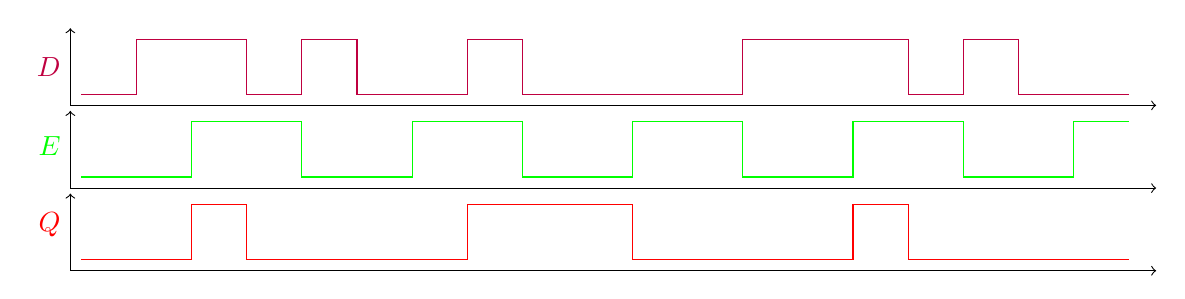
\begin{tikzpicture}[scale=0.7]
      \draw[<->] (-0.2, 1.2) -- (-0.2, -0.2) -- (19.5, -0.2); 
      \draw[<->, yshift=-1.5cm] (-0.2, 1.2) -- (-0.2, -0.2) -- (19.5, -0.2); 
      \draw[<->, yshift=-3cm] (-0.2, 1.2) -- (-0.2, -0.2) -- (19.5, -0.2); 
      \node[purple, left] at (-0.2, 0.5) {$D$}; 
      \node[green, left, yshift=-1cm] at (-0.2, 0.5) {$E$}; 
      \node[red, left, yshift=-2cm] at (-0.2, 0.5) {$Q$}; 

      \draw[purple] (0, 0) -- 
        (1, 0) -- (1, 1) -- (3, 1) -- (3, 0) -- 
        (4, 0) -- (4, 1) -- (5, 1) -- (5, 0) -- 
        (7, 0) -- (7, 1) -- (8, 1) -- (8, 0) -- 
        (12, 0) -- (12, 1) -- (15, 1) -- (15, 0) -- 
        (16, 0) -- (16, 1) -- (17, 1) -- (17, 0) -- 
        (19, 0);
      \draw[green, yshift=-1.5cm] (0, 0) -- 
        (2, 0) -- (2, 1) -- (4, 1) -- (4, 0) -- 
        (6, 0) -- (6, 1) -- (8, 1) -- (8, 0) -- 
        (10, 0) -- (10, 1) -- (12, 1) -- (12, 0) -- 
        (14, 0) -- (14, 1) -- (16, 1) -- (16, 0) -- 
        (18, 0) -- (18, 1) -- (19, 1);
      \draw[red, yshift=-3cm] (0, 0) -- 
        (2, 0) -- (2, 1) -- (3, 1) -- (3, 0) -- 
        (7, 0) -- (7, 1) -- (10, 1) -- (10, 0) -- 
        (14, 0) -- (14, 1) -- (15, 1) -- (15, 0) -- 
        (19, 0);
    \end{tikzpicture}
    \caption{$E$ is connected to a clock that ocsillates at regular intervals.}
  \end{figure}

  This is still not a perfect solution for synchronizing some components. Depending on the frequency of the clock, $E$ may be high for as long at 50 microseconds. That's a long time for the data latch to be open to changes in $D$. For some applications, particularly those where the outputs are fed back to the inputs, we can avoid disorder and noise from $D$ by drastically limiting the amount of time $E$ is open during each clock cycle. 
  
  But simply increasing the frequency of the clock isn't a practical solution, given that a computer contains a mixture of fast and slow components. A more clever solution is to only allow changes to the latch when the clock input $E$ is changing from low to high. Due to propagation delay, this is indeed a feasible solution since the waveforms are not truly square waves. 

  \begin{definition}[Rising, Falling Edge]
    The period when a signal 
    \begin{enumerate}
      \item changes from $0$ to $1$ is called the \textbf{rising edge}. 
      \item changes from $1$ to $0$ is called the \textbf{falling edge}. 
    \end{enumerate}
    This usually takes a few nanoseconds. 

    \begin{figure}[H]
      \centering 
      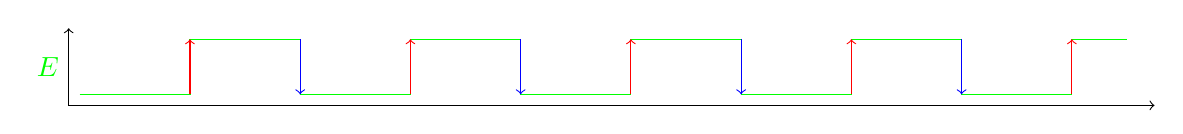
\begin{tikzpicture}[scale=0.7]
        \draw[<->] (-0.2, 1.2) -- (-0.2, -0.2) -- (19.5, -0.2); 
        \node[green, left] at (-0.2, 0.5) {$E$}; 

        \draw[green] (0, 0) -- 
          (2, 0) -- (2, 1) -- (4, 1) -- (4, 0) -- 
          (6, 0) -- (6, 1) -- (8, 1) -- (8, 0) -- 
          (10, 0) -- (10, 1) -- (12, 1) -- (12, 0) -- 
          (14, 0) -- (14, 1) -- (16, 1) -- (16, 0) -- 
          (18, 0) -- (18, 1) -- (19, 1);

        \draw[blue, <-] (4, 0) -- (4, 1); 
        \draw[blue, <-] (8, 0) -- (8, 1); 
        \draw[blue, <-] (12, 0) -- (12, 1); 
        \draw[blue, <-] (16, 0) -- (16, 1); 

        \draw[red, ->] (2, 0) -- (2, 1); 
        \draw[red, ->] (6, 0) -- (6, 1); 
        \draw[red, ->] (10, 0) -- (10, 1); 
        \draw[red, ->] (14, 0) -- (14, 1); 
        \draw[red, ->] (18, 0) -- (18, 1); 
      \end{tikzpicture}
      \caption{Rising edges are in red, falling edges in blue.}
    \end{figure}
  \end{definition}

  As a summary, for level-triggered (transparent) latches, we have active high and active low. Analogously, for edge-triggered latches, we have rising edge and falling edge. We want to build a D-latch that will respond to changes in $D$ \textit{at the rising edge}, with subsequent changes in $D$ being ignored until the next rising edge. 

  \begin{figure}[H]
    \centering
    \begin{subfigure}[b]{0.32\textwidth}
      \centering
      \begin{tikzpicture}[circuit logic US]
        \node[and gate, scale=1.5] (and) at (3, 0) {};
        \node[not gate] (not) at (1, -0.3) {};
        \draw[blue] (-1, 0.2) -- (0, 0.2) -- (0, -0.3) -- (not.input);
        \draw[red] (not.output) -- (and.input 2); 
        \draw[blue] (-1, 0.2) -- (and.input 1); 
        \draw[blue] (and.output) -- (4, 0);
        \fill[blue] (0, 0.2) circle (1.5pt);
      \end{tikzpicture}
      \caption{By default the input current is $0$, and so the top input of the AND gate is $0$ and the bottom is $1$. }
    \end{subfigure}
    \hfill 
    \begin{subfigure}[b]{0.32\textwidth}
      \centering
      \begin{tikzpicture}[circuit logic US]
        \node[and gate, scale=1.5] (and) at (3, 0) {};
        \node[not gate] (not) at (1, -0.3) {};
        \draw[red] (-1, 0.2) -- (0, 0.2) -- (0, -0.3) -- (not.input);
        \draw[red] (not.output) -- (and.input 2); 
        \draw[red] (-1, 0.2) -- (and.input 1); 
        \draw[red] (and.output) -- (4, 0);
        \fill[red] (0, 0.2) circle (1.5pt);
      \end{tikzpicture}
      \caption{If the electric current of $1$ travels through the input wire, the top AND input becomes $1$. There is a small delay where the current does not reach the output of the NOT gate, so the output is $1$. }
    \end{subfigure}
    \hfill 
    \begin{subfigure}[b]{0.32\textwidth}
      \centering
      \begin{tikzpicture}[circuit logic US]
        \node[and gate, scale=1.5] (and) at (3, 0) {};
        \node[not gate] (not) at (1, -0.3) {};
        \draw[red] (-1, 0.2) -- (0, 0.2) -- (0, -0.3) -- (not.input);
        \draw[blue] (not.output) -- (and.input 2); 
        \draw[red] (-1, 0.2) -- (and.input 1); 
        \draw[blue] (and.output) -- (4, 0);
        \fill[red] (0, 0.2) circle (1.5pt);
      \end{tikzpicture}
      \caption{The signal goes through the NOT gate, turning the AND output back to $0$.}
    \end{subfigure}
    \caption{An edge detection device. Note that if we want to delay the signal even further, we can put an arbitrary amount of NAND gates.}
  \end{figure}

  We take this idea to build an edge detection device. 

  \begin{definition}[Edge Detection Device]
    This is a rising edge detection device. Note that depending on many factors, like manufacturing, temperature, etc., there may not be a long enough delay to actually detect an edge, and in this case you can just add more (odd number of ) NOT gates 

    \begin{figure}[H]
      \centering
      \begin{subfigure}[b]{0.48\textwidth}
        \centering
        \begin{tikzpicture}[circuit logic US]
          \node[and gate, scale=1.5] (and) at (3, 0) {};
          \node[not gate] (not) at (1, -0.3) {};
          \draw (-1, 0.2) -- (0, 0.2) -- (0, -0.3) -- (not.input);
          \draw (not.output) -- (and.input 2); 
          \draw (-1, 0.2) -- (and.input 1); 
          \draw (and.output) -- (4, 0);
          \fill (0, 0.2) circle (1.5pt);
        \end{tikzpicture}
        \caption{Positive edge triggered detection device.}
      \end{subfigure}
      \hfill 
      \begin{subfigure}[b]{0.48\textwidth}
        \centering
        \begin{tikzpicture}[circuit logic US]
          \node[nor gate, scale=1.5] (and) at (3, 0) {};
          \node[not gate] (not) at (1, -0.3) {};
          \draw (-1, 0.2) -- (0, 0.2) -- (0, -0.3) -- (not.input);
          \draw (not.output) -- (and.input 2); 
          \draw (-1, 0.2) -- (and.input 1); 
          \draw (and.output) -- (4, 0);
          \fill (0, 0.2) circle (1.5pt);
        \end{tikzpicture}
        \caption{Negative edge triggered detection device.}
      \end{subfigure}
      \caption{}
    \end{figure}

    It has the following waveform. 

    \begin{figure}[H]
      \centering 
      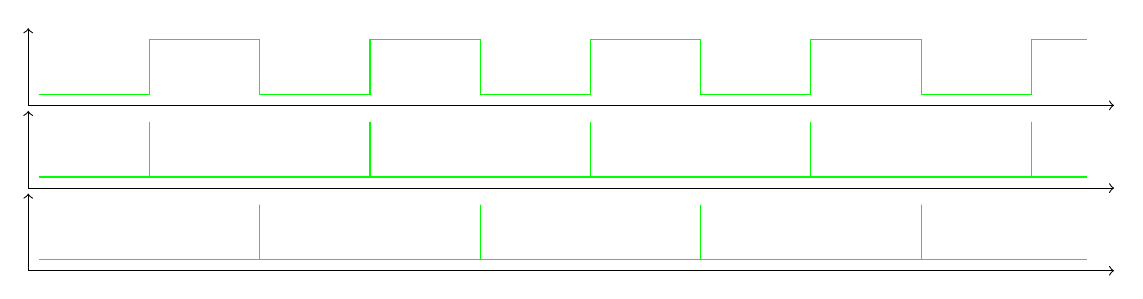
\begin{tikzpicture}[scale=0.7]
        \draw[<->] (-0.2, 1.2) -- (-0.2, -0.2) -- (19.5, -0.2); 
        \draw[<->, yshift=-1.5cm] (-0.2, 1.2) -- (-0.2, -0.2) -- (19.5, -0.2); 
        \draw[<->, yshift=-3cm] (-0.2, 1.2) -- (-0.2, -0.2) -- (19.5, -0.2); 

        \draw[green] (0, 0) -- 
          (2, 0) -- (2, 1) -- (4, 1) -- (4, 0) -- 
          (6, 0) -- (6, 1) -- (8, 1) -- (8, 0) -- 
          (10, 0) -- (10, 1) -- (12, 1) -- (12, 0) -- 
          (14, 0) -- (14, 1) -- (16, 1) -- (16, 0) -- 
          (18, 0) -- (18, 1) -- (19, 1);

        \draw[green, yshift=-1.5cm] (0, 0) -- 
          (2, 0) -- (2, 1) -- (2, 1) -- (2, 0) -- 
          (6, 0) -- (6, 1) -- (6, 1) -- (6, 0) -- 
          (10, 0) -- (10, 1) -- (10, 1) -- (10, 0) -- 
          (14, 0) -- (14, 1) -- (14, 1) -- (14, 0) -- 
          (18, 0) -- (18, 1) -- (18, 1) -- (18, 0) -- 
          (19, 0);

        \draw[green, yshift=-3cm] (0, 0) -- 
          (4, 0) -- (4, 1) -- (4, 0) -- 
          (8, 0) -- (8, 1) -- (8, 0) -- 
          (12, 0) -- (12, 1) -- (12, 0) -- 
          (16, 0) -- (16, 1) -- (16, 0) -- 
          (19, 0);
      \end{tikzpicture}
      \caption{The clock cycle (top). Positive edge detection device (middle). Negative edge detection device (bottom). }
    \end{figure}
  \end{definition}

  Now if we combine our D latch with the edge detection device, we change it from a level-triggered device to an edge-triggered device. Since we are using a clock as our trigger, we also call this a \textit{pulse D-latch}. 

  \begin{definition}[Edge-Triggered D-Latch, Pulse Latch]
    An \textbf{edge-triggered D-latch}, also known as a \textbf{pulse D-latch},\footnote{Often, edge-triggered latches are in general referred to as a flip flop, but we will distinguish that a bit later.} is a D-latch that is enabled on the rising edge of a clock cycle. 

    \begin{figure}[H]
      \centering 
      \begin{tikzpicture}[circuit logic US]
        \node[flipflop D] (D1){};
      \end{tikzpicture}
      \caption{A clocked D latch. Note that the triangle is used to indicate that the clock is inputted. } 
    \end{figure}

    \begin{figure}[H]
      \centering 
      \begin{tikzpicture}[circuit logic US]
        \node[and gate] (and) at (-4, -1.2) {};
        \node[not gate, scale=0.7] (not) at (-5.3, -1.4) {};
        \draw (-6.2, -1.11) -- (and.input 1);
        \draw (-5.8, -1.11) -- (-5.8, -1.4) -- (not.input);
        \fill (-5.8, -1.11) circle (1.5pt); 
        \node[left] at (-6.2, -1.1) {CLK}; 
        \draw(and.output) -- (-3.2, -1.2);
        \draw(not.output) -- (and.input 2); 

        \node[nand gate] (nand1) at (-2, 1.1) {};
        \node[nand gate] (nand2) at (-2, -1.1) {};
        \node[nand gate] (nor1) at (0, 1) {}; 
        \node[nand gate] (nor2) at (0, -1) {}; 

        \draw (-3.5, 1.2) -- (nand1.input 1);
        \draw (-3.5, -1.2) -- (nand2.input 2);
        \node[left] at (-3.5,1.2) {$R$};
        \node[right] at (2, 1) {$Q$};
        \node[right] at (2, -1) {$\overline{Q}$};

        \draw (-3.5, -1.2) -- (-3.2, -1.2) -- (-3.2, 1) -- (nand1.input 2);
        \fill (-3.2, -1.2) circle (1.5pt);
        \draw (nand1.output) -- (-1.2, 1.1) -- (-1.2, 0.9) -- (-2.7, -0.9) -- (-2.7, -1) -- (nand2.input 1);

        \draw (nand1.output) -- (nor1.input 1);
        \draw (nand2.output) -- (nor2.input 2);
        \draw (nor1.output) -- (2, 1); 
        \draw (nor2.output) -- (2, -1); 

        \draw (nor1.output) -- (1.5, 1) -- (1.5, 0.8) -- (-1, -0.7) -- (-1, -0.9) -- (nor2.input 1);
        \draw (nor2.output) -- (1.5, -1) -- (1.5, -0.8) -- (-1, 0.7) -- (-1, 0.9) -- (nor1.input 2);
        \fill (1.5,1) circle (1.5pt);
        \fill (1.5,-1) circle (1.5pt);
      \end{tikzpicture} 
      \caption{} 
    \end{figure}
  \end{definition}

  \begin{example}[Edge-Triggered D-Latch Waveforms]
    \begin{figure}[H]
      \centering 
      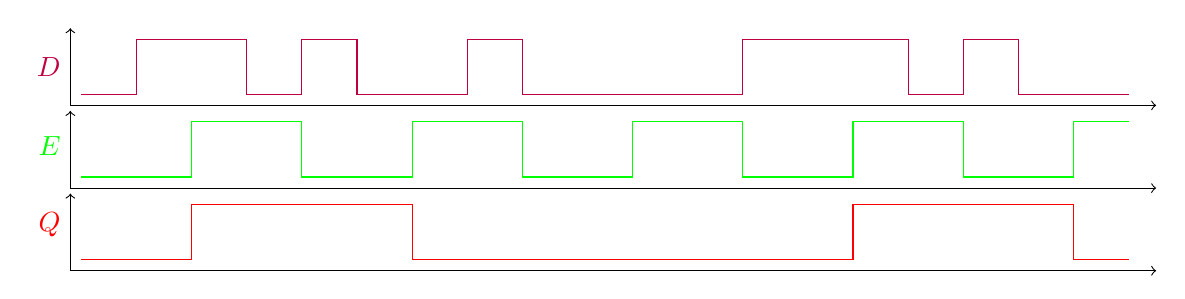
\begin{tikzpicture}[scale=0.7]
        \draw[<->] (-0.2, 1.2) -- (-0.2, -0.2) -- (19.5, -0.2); 
        \draw[<->, yshift=-1.5cm] (-0.2, 1.2) -- (-0.2, -0.2) -- (19.5, -0.2); 
        \draw[<->, yshift=-3cm] (-0.2, 1.2) -- (-0.2, -0.2) -- (19.5, -0.2); 
        \node[purple, left] at (-0.2, 0.5) {$D$}; 
        \node[green, left, yshift=-1cm] at (-0.2, 0.5) {$E$}; 
        \node[red, left, yshift=-2cm] at (-0.2, 0.5) {$Q$}; 

        \draw[purple] (0, 0) -- 
          (1, 0) -- (1, 1) -- (3, 1) -- (3, 0) -- 
          (4, 0) -- (4, 1) -- (5, 1) -- (5, 0) -- 
          (7, 0) -- (7, 1) -- (8, 1) -- (8, 0) -- 
          (12, 0) -- (12, 1) -- (15, 1) -- (15, 0) -- 
          (16, 0) -- (16, 1) -- (17, 1) -- (17, 0) -- 
          (19, 0);
        \draw[green, yshift=-1.5cm] (0, 0) -- 
          (2, 0) -- (2, 1) -- (4, 1) -- (4, 0) -- 
          (6, 0) -- (6, 1) -- (8, 1) -- (8, 0) -- 
          (10, 0) -- (10, 1) -- (12, 1) -- (12, 0) -- 
          (14, 0) -- (14, 1) -- (16, 1) -- (16, 0) -- 
          (18, 0) -- (18, 1) -- (19, 1);
        \draw[red, yshift=-3cm] (0, 0) -- 
          (2, 0) -- (2, 1) -- (6, 1) -- (6, 0) -- 
          (14, 0) -- (14, 1) -- (18, 1) -- (18, 0) --
          (19, 0);
      \end{tikzpicture}
      \caption{Again, we just let the result $Q$ follow the input $D$ whenever $E = 1$,and continue the rest for when $E = 0$.}
    \end{figure}
  \end{example}

  \begin{definition}[Set-Reset Inputs]
    Another enhancement we can make is to have an option to manually set the latch to be either $Q = 1$ or $0$, independent of the clock. This gives us the \textbf{pulse D-latch}, which allows us to initialize it unconditionally. 

    \begin{figure}[H]
      \centering 
      \begin{tikzpicture}
        \node[latch, align=center, add async SR] (latch) at (0,0) {};
      \end{tikzpicture}
      \caption{D latch with asynchronous set/reset.} 
    \end{figure}

    The implementation is to simply add extra inputs after the NAND gates. 

    \begin{figure}[H]
      \centering 
      \begin{tikzpicture}[circuit logic US]
        \node[and gate] (and) at (-4, -1.2) {};
        \node[not gate, scale=0.7] (not) at (-5.3, -1.4) {};
        \draw (-6.2, -1.11) -- (and.input 1);
        \draw (-5.8, -1.11) -- (-5.8, -1.4) -- (not.input);
        \fill (-5.8, -1.11) circle (1.5pt); 
        \node[left] at (-6.2, -1.1) {CLK}; 
        \draw(and.output) -- (-3.2, -1.2);
        \draw(not.output) -- (and.input 2); 

        \node[nand gate] (nand1) at (-2, 1.1) {};
        \node[nand gate] (nand2) at (-2, -1.1) {};
        \node[nand gate, number inputs=3] (nor1) at (0, 1) {}; 
        \node[nand gate, number inputs=3] (nor2) at (0, -1) {}; 

        \draw (-3.5, 1.2) -- (nand1.input 1);
        \draw (-3.5, -1.2) -- (nand2.input 2);
        \node[left] at (-3.5,1.2) {$R$};
        \node[right] at (2, 1) {$Q$};
        \node[right] at (2, -1) {$\overline{Q}$};

        \draw (-3.5, -1.2) -- (-3.2, -1.2) -- (-3.2, 1) -- (nand1.input 2);
        \fill (-3.2, -1.2) circle (1.5pt);
        \draw (nand1.output) -- (-1.2, 1.1) -- (-1.2, 0.9) -- (-2.7, -0.9) -- (-2.7, -1) -- (nand2.input 1);

        \node[above] at (-1.2, 1.8) {SET};
        \node[below] at (-1.2, -1.8) {RESET};
        \draw (-1.2, 1.8) -- (-1.2, 1.2) -- ([yshift=0.1cm]nor1.input 1);
        \draw (-1.2, -1.8) -- (-1.2, -1.2) -- ([yshift=-0.1cm]nor2.input 2);
        \draw (nand1.output) -- (nor1.input 1);
        \draw (nand2.output) -- (nor2.input 2);
        \draw (nor1.output) -- (2, 1); 
        \draw (nor2.output) -- (2, -1); 

        \draw (nor1.output) -- (1.5, 1) -- (1.5, 0.8) -- (-1, -0.7) -- (-1, -0.9) -- (nor2.input 1);
        \draw (nor2.output) -- (1.5, -1) -- (1.5, -0.8) -- (-1, 0.7) -- (-1, 0.9) -- (nor1.input 2);
        \fill (1.5,1) circle (1.5pt);
        \fill (1.5,-1) circle (1.5pt);
      \end{tikzpicture} 
      \caption{} 
    \end{figure}
  \end{definition}

  This gives us a reliable device for storing 1 bit of memory. It is enabled and disabled by a clock signal, and used in registers, memory circuits, and counters as we will see later. 

\subsection{Flip Flops}

  So far, we have considered various mechanisms that allowed for greater control of a latch, along with robustness to noise. Now we revisit the final problem of attempting to \textit{coordinate} a group of latches, where timing is a fundamental consideration. Just like the conductor of an orchestra, the clock sets the timing and the pace of everything in the computer, which consists of both fast and slow moving parts. 

  \begin{figure}[H]
    \centering 
    \begin{tikzpicture}
      \node[draw, circle] (clock) at (-4, -1) {clock};
      \foreach \h in {0, 2, 4} {
        \node[flipflop D, scale=0.5] (D1) at (0.4, 0.6+\h){};
        \draw (D1.pin 3) -- ++(-0.85, 0) -- (-1, -1) -- (clock.east);
        \draw (D1.pin 1) -- ++ (-3, 0);
      }
    \end{tikzpicture}
    \caption{}
  \end{figure}

  Ideally, to synchronize the setting of these latches we'd make all of the inputs the way we want them to be while the clock signal is low. Then, when the clock signal becomes high, these input values would be transmitted to the latches and their values stored. 

  But unwanted fluctuations---known as \textit{glitches}---can occur on the data lines because of propagation delays and even noise.  Conceivably, we can have a situation in which our latches haven't had enough time to achieve their correct values before the clock pulse ends. It is crucial that these inputs are allowed to settle into their correct values while the clock signal is high. This is because there is a different circuit ready to make iemmediate use of the data in the register, even perhaps during the very next clock cycle. The outputs of these latches have to be stable before they are sampled. The data in this register must be accurate before something else reads it. Otherwise, we would have complete garbage outputs. 

  We could try to avoid the problem caused by glitches by speeding up the clock, allowing less time for them to matter, but we also have to allow time for the components to do their jobs. We have to cater for their propagation delays. If a clock is running too quickly, some components won't be able to keep up. 

  We can also make circuits less susceptible to glitches by building edge-triggered devices like pulse latches, but the rising edge of a clock cycle is only in the order of a few nanoseconds, and even with very careful design, there might not be enough time for everything to keep pace. Therefore, the clock period must be so that all of the other circuits have time to stabilize during the same high phase of the same clock cycle. 

  Ultimately, if all circuits in a computer work on the basis that only one signal change per clock cycle matters, then their behavior can be coordinate reliably. One way that we can ensure that this is the case is to build a memory device that is immune to glitches, called the \textit{master-slave D-type flip-flop}. With this, we can precisely control the moment at which a group of them will change state. 

  \begin{definition}[Master-Slave D-Type Flip Flop]
    The \textbf{master-slave D-Type flip-flop (DFF)} consists of two active-high gated latches. The left portion, called the \textit{master}, is a gated D-latch. The right portion, called the \textit{slave}, is a gated SR latch that takes the output of the master as its input and is enabled by the inverse of the clock signal. 

    Taken together, the data and the clock inputs enable to the DFF to implement the time-based behavior 
    \begin{equation}
      \mathrm{out}(t) = \mathrm{in}(t - 1) 
    \end{equation}
    That is, the DFF outputs the input value from the previous time unit. 

    \begin{figure}[H]
      \centering 
      \begin{tikzpicture}[circuit logic US]
        \begin{scope}[xshift=5cm]
          \node[nand gate] (nand13) at (-2, 1.1) {};
          \node[nand gate] (nand24) at (-2, -1.1) {};
          \node[nand gate] (nand14) at (0, 1) {}; 
          \node[nand gate] (nand23) at (0, -1) {}; 
          \node[not gate] (not) at (-5.5, -1.7) {}; 
          \draw[red] (-3, 1.2) -- (nand13.input 1);
          \draw[blue] (-3, -1.2) -- (nand24.input 2);
          \draw[red] (-8.2, -1.2) -- (-8.2, -1.7) -- (not.input); 
          \draw[blue] (not.output) -- (-3.3, -1.7) -- (-3.3, 0) -- (-2.7, 0) -- (-2.7,1) -- (nand13.input 2);
          
          \draw[blue] (-3, 0) -- (-2.7, 0) -- (-2.7,-1) -- (nand24.input 1);
          \node[right] at (2, 1) {$Q$};
          \node[right] at (2, -1) {$\overline{Q}$};
          \draw[red] (nand13.output) -- (nand14.input 1);
          \draw[red] (nand24.output) -- (nand23.input 2);
          \draw[blue] (nand14.output) -- (2, 1); 
          \draw[red] (nand23.output) -- (2, -1); 
          \draw[blue] (nand14.output) -- (1.5, 1) -- (1.5, 0.8) -- (-1, -0.7) -- (-1, -0.9) -- (nand23.input 1);
          \draw[red] (nand23.output) -- (1.5, -1) -- (1.5, -0.8) -- (-1, 0.7) -- (-1, 0.9) -- (nand14.input 2);
          \fill[blue] (1.5,1) circle (1.5pt);
          \fill[red] (1.5,-1) circle (1.5pt);
          \fill[blue] (-2.7,0) circle (1.5pt);
        \end{scope}

        \node[nand gate] (nand1) at (-2, 1.1) {};
        \node[nand gate] (nand2) at (-2, -1.1) {};
        \node[nand gate] (nor1) at (0, 1) {}; 
        \node[nand gate] (nor2) at (0, -1) {}; 

        \draw[red] (-3.5, 1.2) -- (nand1.input 1);
        \draw[red] (-3.5, -1.2) -- (nand2.input 2);
        \node[left] at (-3.5,-1.2) {CLK};
        \node[left] at (-3.5,1.2) {$D$};

        \draw[red] (-3.5, -1.2) -- (-3.2, -1.2) -- (-3.2, 1) -- (nand1.input 2);
        \fill[blue] (-3.2, -1.2) circle (1.5pt);
        \draw[blue] (nand1.output) -- (-1.2, 1.1) -- (-1.2, 0.9) -- (-2.7, -0.9) -- (-2.7, -1) -- (nand2.input 1);

        \draw[blue] (nand1.output) -- (nor1.input 1);
        \draw[red] (nand2.output) -- (nor2.input 2);
        \draw[red] (nor1.output) -- (2, 1) -- (2, 1.2); 
        \draw[blue] (nor2.output) -- (2, -1) -- (2, -1.2); 

        \draw[red] (nor1.output) -- (1.5, 1) -- (1.5, 0.8) -- (-1, -0.7) -- (-1, -0.9) -- (nor2.input 1);
        \draw[blue] (nor2.output) -- (1.5, -1) -- (1.5, -0.8) -- (-1, 0.7) -- (-1, 0.9) -- (nor1.input 2);
        \fill[red] (1.5,1) circle (1.5pt);
        \fill[blue] (1.5,-1) circle (1.5pt);
      \end{tikzpicture} 
      \caption{The master reads the input value $D$ when the clock signal is high (or more specifically, the rising edge of the clock cycle) and latches onto it. Meanwhile, the slave is disabled, so the new output from the flip flop is not available just yet. } 
    \end{figure}

    \begin{figure}[H]
      \centering 
      \begin{tikzpicture}[circuit logic US]
        \begin{scope}[xshift=5cm]
          \node[nand gate] (nand13) at (-2, 1.1) {};
          \node[nand gate] (nand24) at (-2, -1.1) {};
          \node[nand gate] (nand14) at (0, 1) {}; 
          \node[nand gate] (nand23) at (0, -1) {}; 
          \node[not gate] (not) at (-5.5, -1.7) {}; 
          \draw[red] (-3, 1.2) -- (nand13.input 1);
          \draw[blue] (-3, -1.2) -- (nand24.input 2);
          \draw[blue] (-8.2, -1.2) -- (-8.2, -1.7) -- (not.input); 
          \draw[red] (not.output) -- (-3.3, -1.7) -- (-3.3, 0) -- (-2.7, 0) -- (-2.7,1) -- (nand13.input 2);
          
          \draw[red] (-3, 0) -- (-2.7, 0) -- (-2.7,-1) -- (nand24.input 1);
          \node[right] at (2, 1) {$Q$};
          \node[right] at (2, -1) {$\overline{Q}$};
          \draw[blue] (nand13.output) -- (nand14.input 1);
          \draw[red] (nand24.output) -- (nand23.input 2);
          \draw[red] (nand14.output) -- (2, 1); 
          \draw[blue] (nand23.output) -- (2, -1); 
          \draw[red] (nand14.output) -- (1.5, 1) -- (1.5, 0.8) -- (-1, -0.7) -- (-1, -0.9) -- (nand23.input 1);
          \draw[blue] (nand23.output) -- (1.5, -1) -- (1.5, -0.8) -- (-1, 0.7) -- (-1, 0.9) -- (nand14.input 2);
          \fill[red] (1.5,1) circle (1.5pt);
          \fill[blue] (1.5,-1) circle (1.5pt);
          \fill[red] (-2.7,0) circle (1.5pt);
        \end{scope}

        \node[nand gate] (nand1) at (-2, 1.1) {};
        \node[nand gate] (nand2) at (-2, -1.1) {};
        \node[nand gate] (nor1) at (0, 1) {}; 
        \node[nand gate] (nor2) at (0, -1) {}; 

        \draw[red] (-3.5, 1.2) -- (nand1.input 1);
        \draw[blue] (-3.5, -1.2) -- (nand2.input 2);
        \node[left] at (-3.5,-1.2) {CLK};
        \node[left] at (-3.5,1.2) {$D$};

        \draw[blue] (-3.5, -1.2) -- (-3.2, -1.2) -- (-3.2, 1) -- (nand1.input 2);
        \fill[blue] (-3.2, -1.2) circle (1.5pt);
        \draw[red] (nand1.output) -- (-1.2, 1.1) -- (-1.2, 0.9) -- (-2.7, -0.9) -- (-2.7, -1) -- (nand2.input 1);

        \draw[red] (nand1.output) -- (nor1.input 1);
        \draw[red] (nand2.output) -- (nor2.input 2);
        \draw[red] (nor1.output) -- (2, 1) -- (2, 1.2); 
        \draw[blue] (nor2.output) -- (2, -1) -- (2, -1.2); 

        \draw[red] (nor1.output) -- (1.5, 1) -- (1.5, 0.8) -- (-1, -0.7) -- (-1, -0.9) -- (nor2.input 1);
        \draw[blue] (nor2.output) -- (1.5, -1) -- (1.5, -0.8) -- (-1, 0.7) -- (-1, 0.9) -- (nor1.input 2);
        \fill[red] (1.5,1) circle (1.5pt);
        \fill[blue] (1.5,-1) circle (1.5pt);
      \end{tikzpicture} 
      \caption{When the clock cycle falls to low, the slave is enabled, making this an edge triggered device. Data is passed from the master to the slave and is therefore available at the output. } 
    \end{figure}
  \end{definition}

  Essentially a DFF is analogous to an airlock consisting of two doors that can never be both open at the same time. The flip flop is never open so an input signal cannot pass straight through like a regular D latch. The output of the flip flop occurs during the next phase of the same clock cycle. 

  \begin{example}[Waveforms of DFF]
    Let's look at an example where a regular D latch would be insufficient, but a DFF fixes the problem. Note that $Q_m$ behaves just like a D-latch since it is.
    \begin{enumerate}
      \item $t = 2$. $C$ has a rising edge and $D = 0$, so $Q_m = 0$. 
      \item $t = 5$. $D$ has become high, presumably because we want the output at $Q_m$ to go high. But because $C = 0$, this doesn't happen just yet, and the master is still latched in a low state. 
      \item $t = 6$. When $C = 1$, $Q_m$ reacts immediately to follow $D$, and so it becomes high. 
      \item $t = 8$. When $C$ goes low again, $D$ is high and so is $Q_m$, and so the master is latched in a high state. 
      \item $t = 9$. $D$ goes low again, presumably because we want to change the state of the master latch back to low again. But because $C$ is low, $Q_m$ does not follow. 
      \item $t = 10$. When $C$ goes high, $Q_m$ immediately goes low. 
      \item $t = 11$. We can see $D$ changing again while the clock is high. Suppose that a completely different circuit depended on the output of $Q_m$ being low. Since $Q_m$ was both low and then high in the same high clock cycle, the circuit might have missed its chance to read from $Q_m$. We want to avoid this, and ideally, we want to (1) set the value of $D$ \textit{before} the clock goes high, and (2) \textit{not} have $D$ change in the middle of a clock high cycle. \item $t = 12$. Now $C$ is low, and the master is latched in a high state. 
      \item $t = 22$. We can see that the value of $D$ is changing again during a high phase of the clock cycle---another glitch. 
    \end{enumerate}
    If we take a look at the output of the slave $Q_s$, which follows $Q_m$ since the master's output is the slave's input. But more importantly, $Q_s$ only follows $Q_m$ while $C$ is low (because the slave is being fed the inverse of the clock signal). 

    \begin{enumerate}
      \item $t = 6$. $Q_m$ is changing from low to high, but $Q_s$ remains low since $C$ is high. While the flip flop is responding to a change in input, the output remains the same. 
      \item $t = 8$. At the falling edge of the clock cycle, $Q_s$ follows $Q_m$ to become high. Notice that the master's output $Q_m$ cannot be changed now because $C$ is low. This means that changes to the input of the flip-flop cannot impact the output at this point. 
      \item $t = 9$. The input at $D$ has changed from high to low, as if in readiness for another change to the state of the flip flop. 
      \item $t = 10$. When $C$ goes high, the output of the master $Q_m$ changes but this has no impact on $Q_s$. The slave isn't listening. 
      \item $t = 11$. $D$ goes high again during the high phase of the clock cycle. But this glitch has no effect on the output of the flip flop. 
      \item $t = 20$. We see $Q_s$ changing again to follow $Q_m$ while the clock signal is low. The master will also ignore any changes in the input while the flip flop's output is made available. 
      \item $t = 21$. We see $D$ goes high, as if to set the state of the flip-flop to high on the next high cycle. 
      \item $t = 22$. When the clock goes high, $Q_m$ follows $D$ to become high as well. 
      \item $t = 23$. But the input $D$ falls to low while the clock is high, and so does $Q_m$. 
      \item $t = 24$. By the time the clock falls to low again, and the slave is once again responding to changes to its input, the flip flop has ignore yet another glitch. 
    \end{enumerate}

    In summary, the DFF effectively ignores any input fluctuations because the master and slave are enabled on opposite phases of the clock cycle. It is safe because it allows sufficient time for propagation delays and therefore time for the inputs to change and settle down without affecting the output. It is however more complicated and resource-intensive than regular latches. 

    \begin{figure}[H]
      \centering 
      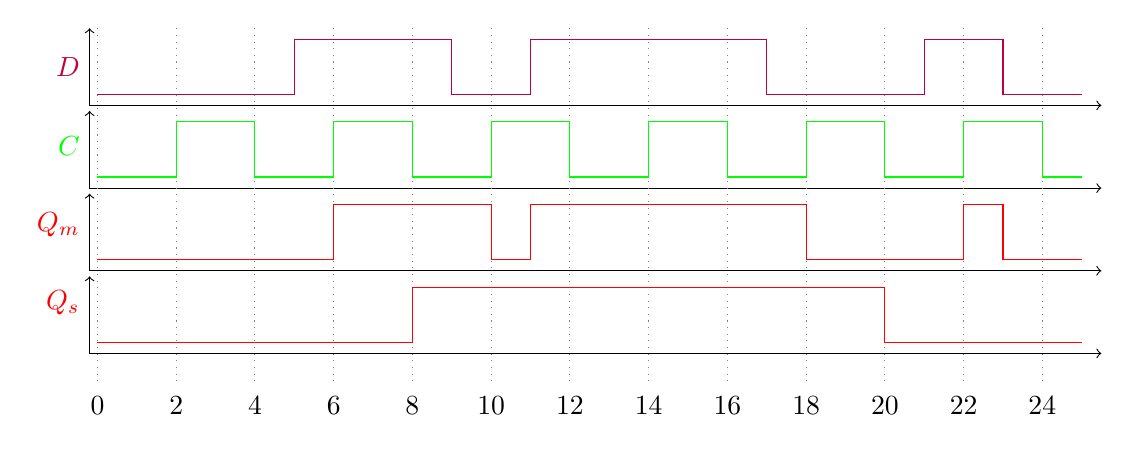
\begin{tikzpicture}[xscale=0.5, yscale=0.7]
        \draw[<->] (-0.2, 1.2) -- (-0.2, -0.2) -- (25.5, -0.2); 
        \draw[<->, yshift=-1.5cm] (-0.2, 1.2) -- (-0.2, -0.2) -- (25.5, -0.2); 
        \draw[<->, yshift=-3cm] (-0.2, 1.2) -- (-0.2, -0.2) -- (25.5, -0.2); 
        \draw[<->, yshift=-4.5cm] (-0.2, 1.2) -- (-0.2, -0.2) -- (25.5, -0.2); 
        
        % Time labels and dotted lines for bottom graph only
        \foreach \x in {0, 2, 4, 6, 8, 10, 12, 14, 16, 18, 20, 22, 24} {
          \draw[dotted, gray] (\x, 1.2) -- (\x, -5.3);
          \node[below] at (\x, -5.3) {\x};
        }
        
        \node[purple, left] at (-0.2, 0.5) {$D$}; 
        \node[green, left, yshift=-1cm] at (-0.2, 0.5) {$C$}; 
        \node[red, left, yshift=-2cm] at (-0.2, 0.5) {$Q_m$}; 
        \node[red, left, yshift=-3cm] at (-0.2, 0.5) {$Q_s$}; 
        
        \draw[purple] (0, 0) -- 
          (5, 0) -- (5, 1) -- (9, 1) -- (9, 0) -- 
          (11, 0) -- (11, 1) -- (17, 1) -- (17, 0) -- 
          (21, 0) -- (21, 1) -- (23, 1) -- (23, 0) -- 
          (25, 0);
        \draw[green, yshift=-1.5cm] (0, 0) -- 
          (2, 0) -- (2, 1) -- (4, 1) -- (4, 0) -- 
          (6, 0) -- (6, 1) -- (8, 1) -- (8, 0) -- 
          (10, 0) -- (10, 1) -- (12, 1) -- (12, 0) -- 
          (14, 0) -- (14, 1) -- (16, 1) -- (16, 0) -- 
          (18, 0) -- (18, 1) -- (20, 1) -- (20, 0) -- 
          (22, 0) -- (22, 1) -- (24, 1) -- (24, 0) -- 
          (25, 0); 
        \draw[red, yshift=-3cm] (0, 0) -- 
          (6, 0) -- (6, 1) -- (10, 1) -- (10, 0) -- 
          (11, 0) -- (11, 1) -- (18, 1) -- (18, 0) -- 
          (22, 0) -- (22, 1) -- (23, 1) -- (23, 0) -- 
          (25, 0); 
        \draw[red, yshift=-4.5cm] (0, 0) -- 
          (8, 0) -- (8, 1) -- (20, 1) -- (20, 0) -- 
          (25, 0);
      \end{tikzpicture}
      \caption{}
    \end{figure}
  \end{example}
  
  Now let's look at two more types of flip-flops. We revisit the problem of invalid states for SR latches, which lead to race conditions (both 1s for active high and both 0s for active low). We introduce the JK latch, which is not a flip flop yet. Note that you put a pulse through $K$ to reset $Q = 0$, and a pulse through $J$ to set $Q = 1$.

  \begin{figure}[H]
    \centering
    \begin{subfigure}[b]{0.48\textwidth}
      \centering
      \begin{tikzpicture}[circuit logic US]
        \node[nand gate] (nand1) at (-2, 1.1) {};
        \node[nand gate] (nand2) at (-2, -1.1) {};
        \node[nor gate] (nor1) at (0, 1) {}; 
        \node[nor gate] (nor2) at (0, -1) {}; 

        \draw[red] (-3, 1.0) -- (nand1.input 2);
        \draw[red] (-3, -1.0) -- (nand2.input 1);
        \node[left] at (-3,1.0) {$K$};
        \node[left] at (-3,-1.0) {$J$};
        \node[right] at (2, 1) {$Q$};
        \node[right] at (2, -1) {$\overline{Q}$};

        \draw[red] (nand1.input 1) -- (-2.8, 1.2) -- (-2.8, 1.6) -- (1.2, 1.6) -- (1.2, 1); 
        \draw[blue] (nand2.input 2) -- (-2.8, -1.2) -- (-2.8, -1.6) -- (1.2, -1.6) -- (1.2, -1); 

        \draw[red] (nand1.output) -- (nor1.input 1);
        \draw[blue] (nand2.output) -- (nor2.input 2);
        \draw[red] (nor1.output) -- (2, 1); 
        \draw[blue] (nor2.output) -- (2, -1); 

        \draw[red] (nor1.output) -- (1.5, 1) -- (1.5, 0.8) -- (-1, -0.7) -- (-1, -0.9) -- (nor2.input 1);
        \draw[blue] (nor2.output) -- (1.5, -1) -- (1.5, -0.8) -- (-1, 0.7) -- (-1, 0.9) -- (nor1.input 2);
        \fill[red] (1.5,1) circle (1.5pt);
        \fill[blue] (1.5,-1) circle (1.5pt);
      \end{tikzpicture} 
      \caption{}
    \end{subfigure}
    \hfill 
    \begin{subfigure}[b]{0.48\textwidth}
      \centering
      \begin{tikzpicture}[circuit logic US]
        \node[nand gate] (nand1) at (-2, 1.1) {};
        \node[nand gate] (nand2) at (-2, -1.1) {};
        \node[nor gate] (nor1) at (0, 1) {}; 
        \node[nor gate] (nor2) at (0, -1) {}; 

        \draw[red] (-3, 1.0) -- (nand1.input 2);
        \draw[red] (-3, -1.0) -- (nand2.input 1);
        \node[left] at (-3,1.0) {$K$};
        \node[left] at (-3,-1.0) {$J$};
        \node[right] at (2, 1) {$Q$};
        \node[right] at (2, -1) {$\overline{Q}$};

        \draw[blue] (nand1.input 1) -- (-2.8, 1.2) -- (-2.8, 1.6) -- (1.2, 1.6) -- (1.2, 1); 
        \draw[red] (nand2.input 2) -- (-2.8, -1.2) -- (-2.8, -1.6) -- (1.2, -1.6) -- (1.2, -1); 

        \draw[blue] (nand1.output) -- (nor1.input 1);
        \draw[red] (nand2.output) -- (nor2.input 2);
        \draw[blue] (nor1.output) -- (2, 1); 
        \draw[red] (nor2.output) -- (2, -1); 

        \draw[blue] (nor1.output) -- (1.5, 1) -- (1.5, 0.8) -- (-1, -0.7) -- (-1, -0.9) -- (nor2.input 1);
        \draw[red] (nor2.output) -- (1.5, -1) -- (1.5, -0.8) -- (-1, 0.7) -- (-1, 0.9) -- (nor1.input 2);
        \fill[blue] (1.5,1) circle (1.5pt);
        \fill[red] (1.5,-1) circle (1.5pt);
      \end{tikzpicture} 
      \caption{}
    \end{subfigure}
    \caption{JK active high latch. When you set $J = K = 1$, the latch oscillates between $Q = 0$ and $Q = 1$ very fast, but this eliminates the possibility where $Q$ is both $1$ or both $0$.}
  \end{figure}

  Note that we can do the same with an active low JK latch, which will be functionally identical to the active high one. Now we are a step closer to the JK flip flop.  

  \begin{definition}[Level Triggered JK Flip-Flop]
    By adding a gate/enabler and synching it with the clock, we can get the \textbf{level triggered JK flip flop}. 

    \begin{figure}[H]
      \centering 
      \begin{tikzpicture}[circuit logic US]
        \node[nand gate] (nand1) at (-2, 1.1) {};
        \node[nand gate] (nand2) at (-2, -1.1) {};
        \node[nor gate] (nor1) at (0, 1) {}; 
        \node[nor gate] (nor2) at (0, -1) {}; 
        \draw (-3, 0) -- (-2.7, 0) -- (-2.7, 0.9) -- ([yshift=-0.1cm]nand1.input 2); 
        \draw (-3, 0) -- (-2.7, 0) -- (-2.7, -0.9) -- ([yshift=0.1cm]nand2.input 1); 

        \draw[] (-3, 1.0) -- (nand1.input 2);
        \draw[] (-3, -1.0) -- (nand2.input 1);
        \node[left] at (-3,1.0) {$K$};
        \node[left] at (-3,-1.0) {$J$};
        \node[left] at (-3,0) {CLK};
        \node[right] at (2, 1) {$Q$};
        \node[right] at (2, -1) {$\overline{Q}$};

        \draw[] (nand1.input 1) -- (-2.8, 1.2) -- (-2.8, 1.6) -- (1.2, 1.6) -- (1.2, 1); 
        \draw[] (nand2.input 2) -- (-2.8, -1.2) -- (-2.8, -1.6) -- (1.2, -1.6) -- (1.2, -1); 

        \draw[] (nand1.output) -- (nor1.input 1);
        \draw[] (nand2.output) -- (nor2.input 2);
        \draw[] (nor1.output) -- (2, 1); 
        \draw[] (nor2.output) -- (2, -1); 

        \draw[] (nor1.output) -- (1.5, 1) -- (1.5, 0.8) -- (-1, -0.7) -- (-1, -0.9) -- (nor2.input 1);
        \draw[] (nor2.output) -- (1.5, -1) -- (1.5, -0.8) -- (-1, 0.7) -- (-1, 0.9) -- (nor1.input 2);
        \fill[] (1.5,1) circle (1.5pt);
        \fill[] (1.5,-1) circle (1.5pt);
      \end{tikzpicture} 
      \caption{Level Triggered JK Flip Flop. } 
    \end{figure}
  \end{definition}

  \begin{example}[Waveforms of Level Triggered JK Flip Flop]
    Let's go through the timing diagram. 
    \begin{enumerate}
      \item $t = 1$. When $K = 1$, there is no change in $Q$ since the clock is low. The flip flop is disabled. 
      \item $t = 2$. The clock is high and the reset signal goes through the AND gate, and $Q = 0$. 
      \item $t = 10$. $J$ becomes high and the clock is high, enabling the latch again, and consequently $Q$ is high again. 
      \item $t = 18, 22, 26$. When $C, J, K$ are all high, then the circuit begins to oscillate uncontrollably.  
    \end{enumerate}

    \begin{figure}[H]
      \centering 
      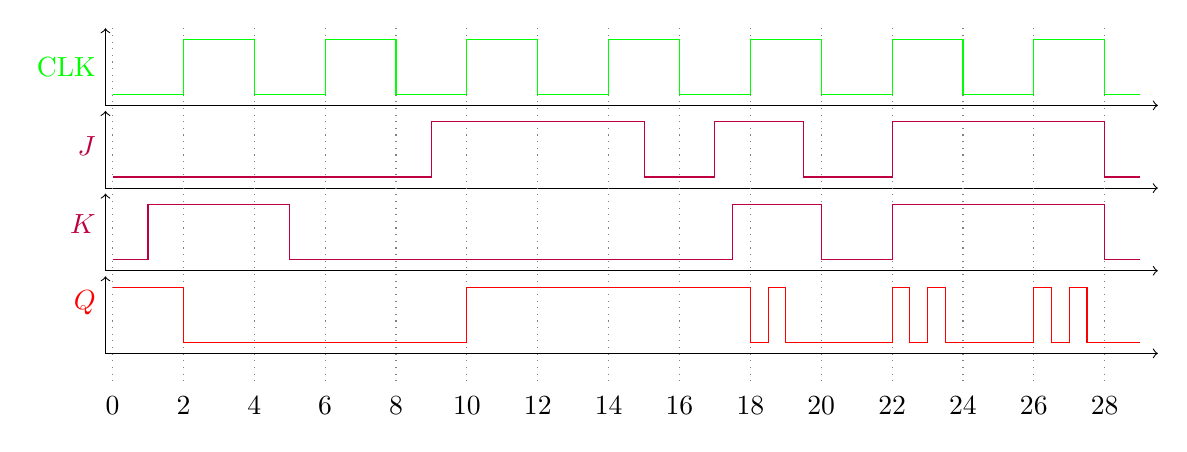
\begin{tikzpicture}[xscale=0.45, yscale=0.7]
        \draw[<->] (-0.2, 1.2) -- (-0.2, -0.2) -- (29.5, -0.2); 
        \draw[<->, yshift=-1.5cm] (-0.2, 1.2) -- (-0.2, -0.2) -- (29.5, -0.2); 
        \draw[<->, yshift=-3cm] (-0.2, 1.2) -- (-0.2, -0.2) -- (29.5, -0.2); 
        \draw[<->, yshift=-4.5cm] (-0.2, 1.2) -- (-0.2, -0.2) -- (29.5, -0.2); 
        
        % Time labels and dotted lines for bottom graph only
        \foreach \x in {0, 2, 4, 6, 8, 10, 12, 14, 16, 18, 20, 22, 24, 26, 28} {
          \draw[dotted, gray] (\x, 1.2) -- (\x, -5.3);
          \node[below] at (\x, -5.3) {\x};
        }
        
        \node[green, left] at (-0.2, 0.5) {CLK}; 
        \node[purple, left, yshift=-1cm] at (-0.2, 0.5) {$J$}; 
        \node[purple, left, yshift=-2cm] at (-0.2, 0.5) {$K$}; 
        \node[red, left, yshift=-3cm] at (-0.2, 0.5) {$Q$}; 
        
        \draw[green] (0, 0) -- 
          (2, 0) -- (2, 1) -- (4, 1) -- (4, 0) -- 
          (6, 0) -- (6, 1) -- (8, 1) -- (8, 0) -- 
          (10, 0) -- (10, 1) -- (12, 1) -- (12, 0) -- 
          (14, 0) -- (14, 1) -- (16, 1) -- (16, 0) -- 
          (18, 0) -- (18, 1) -- (20, 1) -- (20, 0) -- 
          (22, 0) -- (22, 1) -- (24, 1) -- (24, 0) -- 
          (26, 0) -- (26, 1) -- (28, 1) -- (28, 0) -- 
          (29, 0); 
        \draw[purple, yshift=-1.5cm] (0, 0) -- 
          (9, 0) -- (9, 1) -- (15, 1) -- (15, 0) -- 
          (17, 0) -- (17, 1) -- (19.5, 1) -- (19.5, 0) -- 
          (22, 0) -- (22, 1) -- (28, 1) -- (28, 0) -- 
          (29, 0); 
        \draw[purple, yshift=-3cm] (0, 0) -- 
          (1, 0) -- (1, 1) -- (5, 1) -- (5, 0) -- 
          (17.5, 0) -- (17.5, 1) -- (20, 1) -- (20, 0) -- 
          (22, 0) -- (22, 1) -- (28, 1) -- (28, 0) -- 
          (29, 0); 
        \draw[red, yshift=-4.5cm] 
          (0, 1) -- (2, 1) -- (2, 0) -- 
          (10, 0) -- (10, 1) -- (18, 1) -- (18, 0) --
          (18.5, 0) -- (18.5, 1) -- (19, 1) -- (19, 0) --
          (22, 0) -- (22, 1) -- (22.5, 1) -- (22.5, 0) -- 
          (23, 0) -- (23, 1) -- (23.5, 1) -- (23.5, 0) -- 
          (26, 0) -- (26, 1) -- (26.5, 1) -- (26.5, 0) -- 
          (27, 0) -- (27, 1) -- (27.5, 1) -- (27.5, 0) -- 
          (29, 0);
      \end{tikzpicture}
      \caption{}
    \end{figure}
  \end{example}

  To take advantage of this oscillation, we need a flip flop that will only react the inputs while the clock singal is changing from low to high, i.e. on the rising edge. 

  \begin{definition}[Edge Triggered JK Flip Flop]
    To fix the weird oscillation issues, we can use the edge detection device to get the \textbf{edge triggered JK flip-flop}. 

    \begin{figure}[H]
      \centering 
      \begin{tikzpicture}[circuit logic US]
        \node[and gate] (and) at (-4, 0) {};
        \node[not gate, scale=0.7] (not) at (-5.3, -0.2) {};
        \draw (-6.2, 0.09) -- (and.input 1);
        \draw (-5.8, 0.09) -- (-5.8, -0.2) -- (not.input);
        \fill (-5.8, 0.09) circle (1.5pt); 
        \node[left] at (-6.2, 0.2) {CLK}; 
        \draw(and.output) -- (-2.7, 0);
        \draw(not.output) -- (and.input 2); 

        \node[nand gate] (nand1) at (-2, 1.1) {};
        \node[nand gate] (nand2) at (-2, -1.1) {};
        \node[nor gate] (nor1) at (0, 1) {}; 
        \node[nor gate] (nor2) at (0, -1) {}; 
        \draw (-3, 0) -- (-2.7, 0) -- (-2.7, 0.9) -- ([yshift=-0.1cm]nand1.input 2); 
        \draw (-3, 0) -- (-2.7, 0) -- (-2.7, -0.9) -- ([yshift=0.1cm]nand2.input 1); 

        \draw[] (-3, 1.0) -- (nand1.input 2);
        \draw[] (-3, -1.0) -- (nand2.input 1);
        \node[left] at (-3,1.0) {$K$};
        \node[left] at (-3,-1.0) {$J$};
        \node[right] at (2, 1) {$Q$};
        \node[right] at (2, -1) {$\overline{Q}$};

        \draw[] (nand1.input 1) -- (-2.8, 1.2) -- (-2.8, 1.6) -- (1.2, 1.6) -- (1.2, 1); 
        \draw[] (nand2.input 2) -- (-2.8, -1.2) -- (-2.8, -1.6) -- (1.2, -1.6) -- (1.2, -1); 

        \draw[] (nand1.output) -- (nor1.input 1);
        \draw[] (nand2.output) -- (nor2.input 2);
        \draw[] (nor1.output) -- (2, 1); 
        \draw[] (nor2.output) -- (2, -1); 

        \draw[] (nor1.output) -- (1.5, 1) -- (1.5, 0.8) -- (-1, -0.7) -- (-1, -0.9) -- (nor2.input 1);
        \draw[] (nor2.output) -- (1.5, -1) -- (1.5, -0.8) -- (-1, 0.7) -- (-1, 0.9) -- (nor1.input 2);
        \fill[] (1.5,1) circle (1.5pt);
        \fill[] (1.5,-1) circle (1.5pt);
      \end{tikzpicture} 
      \caption{Edge Triggered JK Flip Flop. } 
    \end{figure}
  \end{definition}

  It is also called the \textit{universal programmable flip flop} since you can make other types of flip flops from JK flip flops. 

  \begin{example}[Waveforms of Edge Triggered JK Flip Flop]
    With the edge detector, only the rising edge of each clock pulse has any effect. Notice that when $J$ and $K$ are both high, a clock pulse will cause the flip flop to toggle from one state to the other (at times $t = 18, 22, 26$).  

    \begin{figure}[H]
      \centering 
      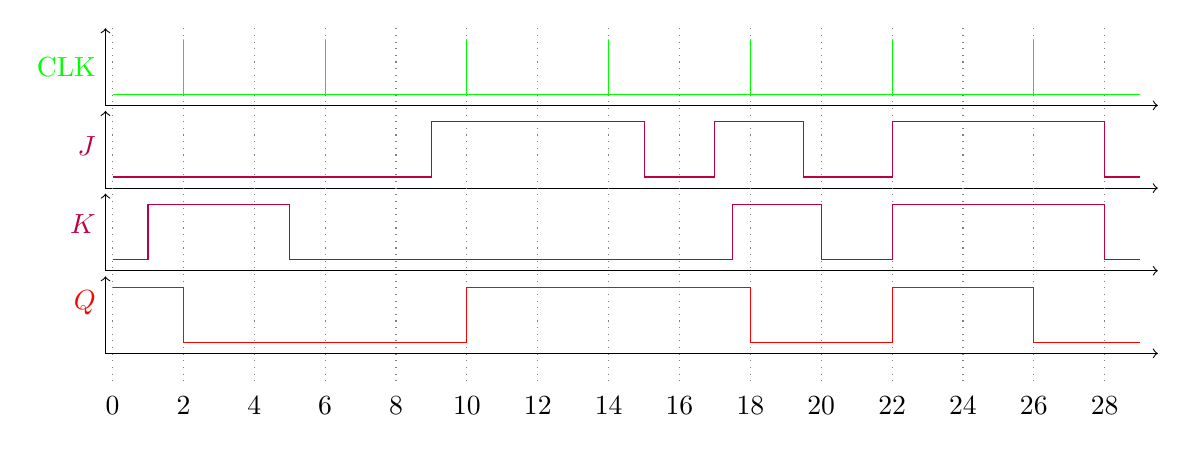
\begin{tikzpicture}[xscale=0.45, yscale=0.7]
        \draw[<->] (-0.2, 1.2) -- (-0.2, -0.2) -- (29.5, -0.2); 
        \draw[<->, yshift=-1.5cm] (-0.2, 1.2) -- (-0.2, -0.2) -- (29.5, -0.2); 
        \draw[<->, yshift=-3cm] (-0.2, 1.2) -- (-0.2, -0.2) -- (29.5, -0.2); 
        \draw[<->, yshift=-4.5cm] (-0.2, 1.2) -- (-0.2, -0.2) -- (29.5, -0.2); 
        
        % Time labels and dotted lines for bottom graph only
        \foreach \x in {0, 2, 4, 6, 8, 10, 12, 14, 16, 18, 20, 22, 24, 26, 28} {
          \draw[dotted, gray] (\x, 1.2) -- (\x, -5.3);
          \node[below] at (\x, -5.3) {\x};
        }
        
        \node[green, left] at (-0.2, 0.5) {CLK}; 
        \node[purple, left, yshift=-1cm] at (-0.2, 0.5) {$J$}; 
        \node[purple, left, yshift=-2cm] at (-0.2, 0.5) {$K$}; 
        \node[red, left, yshift=-3cm] at (-0.2, 0.5) {$Q$}; 
        
        \draw[green] (0, 0) -- 
          (2, 0) -- (2, 1) -- (2, 0) -- (4, 0) -- 
          (6, 0) -- (6, 1) -- (6, 0) -- (8, 0) -- 
          (10, 0) -- (10, 1) -- (10, 0) -- (12, 0) -- 
          (14, 0) -- (14, 1) -- (14, 0) -- (16, 0) -- 
          (18, 0) -- (18, 1) -- (18, 0) -- (20, 0) -- 
          (22, 0) -- (22, 1) -- (22, 0) -- (24, 0) -- 
          (26, 0) -- (26, 1) -- (26, 0) -- (28, 0) -- 
          (29, 0); 
        \draw[purple, yshift=-1.5cm] (0, 0) -- 
          (9, 0) -- (9, 1) -- (15, 1) -- (15, 0) -- 
          (17, 0) -- (17, 1) -- (19.5, 1) -- (19.5, 0) -- 
          (22, 0) -- (22, 1) -- (28, 1) -- (28, 0) -- 
          (29, 0); 
        \draw[purple, yshift=-3cm] (0, 0) -- 
          (1, 0) -- (1, 1) -- (5, 1) -- (5, 0) -- 
          (17.5, 0) -- (17.5, 1) -- (20, 1) -- (20, 0) -- 
          (22, 0) -- (22, 1) -- (28, 1) -- (28, 0) -- 
          (29, 0); 
        \draw[red, yshift=-4.5cm] 
          (0, 1) -- (2, 1) -- (2, 0) -- 
          (10, 0) -- (10, 1) -- (18, 1) -- (18, 0) --
          (22, 0) -- (22, 1) -- (26, 1) -- (26, 0) -- 
          (29, 0);
      \end{tikzpicture}
      \caption{}
    \end{figure}
  \end{example}

  Another simple modification of the JK flip flop gives us another type of flip flop. B simply connecting together $J$ and $K$ to make one input, we now have a device that will toggle from one state to the other when the input is high at the rising edge of the clock. 

  \begin{definition}[Toggle Flip Flip]
    The \textbf{toggle flip-flop}, also known as the \textbf{T-Type flip-flop}, is used as an oscillator (?). 

    \begin{figure}[H]
      \centering 
      \begin{tikzpicture}[circuit logic US]
        \node[and gate] (and) at (-4, 0) {};
        \node[not gate, scale=0.7] (not) at (-5.3, -0.2) {};
        \draw (-6.2, 0.09) -- (and.input 1);
        \draw (-5.8, 0.09) -- (-5.8, -0.2) -- (not.input);
        \fill (-5.8, 0.09) circle (1.5pt); 
        \node[left] at (-6.2, 0.2) {CLK}; 
        \draw(and.output) -- (-2.7, 0);
        \draw(not.output) -- (and.input 2); 

        \node[nand gate] (nand1) at (-2, 1.1) {};
        \node[nand gate] (nand2) at (-2, -1.1) {};
        \node[nor gate] (nor1) at (0, 1) {}; 
        \node[nor gate] (nor2) at (0, -1) {}; 
        \draw (-3, 0) -- (-2.7, 0) -- (-2.7, 0.9) -- ([yshift=-0.1cm]nand1.input 2); 
        \draw (-3, 0) -- (-2.7, 0) -- (-2.7, -0.9) -- ([yshift=0.1cm]nand2.input 1); 

        \draw[] (-3.5, -1.0) -- (-3, -1.0) -- (-3, -0.1) -- (-3.1, 0) -- (-3, 0.1) -- (-3, 1.0) -- (nand1.input 2); 
        \draw[] (-3.5, -1.0) -- (nand2.input 1);
        \node[left] at (-3.5,-1.0) {$T$};
        \node[right] at (2, 1) {$Q$};
        \node[right] at (2, -1) {$\overline{Q}$};

        \draw[] (nand1.input 1) -- (-2.8, 1.2) -- (-2.8, 1.6) -- (1.2, 1.6) -- (1.2, 1); 
        \draw[] (nand2.input 2) -- (-2.8, -1.2) -- (-2.8, -1.6) -- (1.2, -1.6) -- (1.2, -1); 

        \draw[] (nand1.output) -- (nor1.input 1);
        \draw[] (nand2.output) -- (nor2.input 2);
        \draw[] (nor1.output) -- (2, 1); 
        \draw[] (nor2.output) -- (2, -1); 

        \draw[] (nor1.output) -- (1.5, 1) -- (1.5, 0.8) -- (-1, -0.7) -- (-1, -0.9) -- (nor2.input 1);
        \draw[] (nor2.output) -- (1.5, -1) -- (1.5, -0.8) -- (-1, 0.7) -- (-1, 0.9) -- (nor1.input 2);
        \fill[] (1.5,1) circle (1.5pt);
        \fill[] (1.5,-1) circle (1.5pt);
      \end{tikzpicture} 
      \caption{Toggle flip flop. } 
    \end{figure}
  \end{definition} 
  
\subsection{Registers}

  The DFF then unlocks the our first type of memory. 

  \begin{definition}[Register]
    A \textbf{$w$-bit register} is a memory device, composed up of $w$ DFFs, that can hold $w$ bits of memory. It supports 
    \begin{enumerate}
      \item \textit{Read}. 
      \item \textit{Write}. 
    \end{enumerate}

    \begin{figure}[H]
      \centering 
      \begin{tikzpicture}[circuit logic US, yscale=0.7, xscale=0.65]
        \foreach \x [count=\i from 0] in {0, 5, 10, 15} {
          \node[latch, align=center, scale=0.8] (latch) at (\x,0) {};
          \draw (latch.pin 1) -- ++(-0.5,0) node[left] {} -- ++ (0, 1.5) node[above] {in\i}; 
          \draw (latch.pin 3) -- ++(-0.5,0) node[left] {} -- ++ (0, -1) -- (-2, -1.95); 
          \fill (-1.8 + \x, -1.95) circle (2.5pt);
          \draw (latch.pin 6) -- ++(0.5,0) node[right] {} -- ++ (0, -4) node[below] {out\i};
        }
        \node[and gate, scale=1.5] (and) at (-2.8, -1.95) {}; 
        \draw (and.output) -- (-1.8, -1.95);
        
        \node[left] (clk) at (-3.8, -1.75) {CLK};
        \node[left] (load) at (-3.8, -2.15) {load}; 
        \draw (clk.east) -- (and.input 1); 
        \draw (load.east) -- (and.input 2);
      \end{tikzpicture}
      \caption{4-bit register. Since $\overline{Q}$ is redundant we do not consider it as an output in our register. } 
    \end{figure}
  \end{definition}

  So we now have the flexibility to construct memory of arbitrary size. The general convention is to make the registers multiples of 2. 

  \begin{definition}[Word]
    The \textbf{word size} of a register $w$ is the number of bits it can hold. 
    \begin{enumerate}
      \item $8$-bit and $16$-bit registers were used in the early days of computing. 
      \item $32$-bit personal computers were introduced in the 1980s, but they are mostly considered obsolete as of 2025. These machines are known as \textit{32-bit machines}. 
      \item $64$-bit personal computers are the most dominant, known as \textit{64-bit machines}. 
    \end{enumerate}
  \end{definition} 

  It is sort of understandable that making word sizes as power of 2 makes things a bit more convenient. They can be stacked and grouped together conveniently, giving us the following familiar terms of Byte, word, quad, long, etc. Using hexadecimal notation makes them easier to read. 

\subsection{Applications}
  
  \begin{definition}[Divide by 2 Chip]
    The \textbf{divide-by-2 chip} simply splits the frequency of the clock input by 2. It is implemented with a pulse latch---i.e. an edge-triggered D-latch. 

    \begin{figure}[H]
      \centering 
      \begin{tikzpicture}[circuit logic US]
        \node[flipflop D] (D){}; 
        \draw (D.pin 4) -- ++(0.2, 0) -- ++(0, 2.5) -- ++(-2.5, 0) -- ++(0, -0.7) -- (D.pin 1);
        \draw (D.pin 6) -- ++(1,0) node[right] {};
        \draw (D.pin 3) -- ++(-0.5,0) node[left] {CLK};
      \end{tikzpicture}
      \caption{The output $\overline{Q}$ gets rewired into the input $D$, causing the frequency to slow down.}
    \end{figure}
  \end{definition}

  \begin{example}[Waveforms of Divide by 2 Latch]
    The way the divide-by-2 chip acts on a clock waveform is pretty straightforward. 

    \begin{figure}[H]
      \centering 
      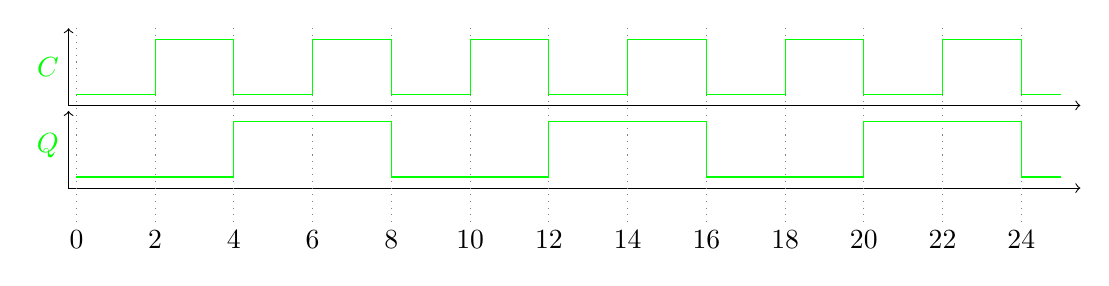
\begin{tikzpicture}[xscale=0.5, yscale=0.7]
        \draw[<->] (-0.2, 1.2) -- (-0.2, -0.2) -- (25.5, -0.2); 
        \draw[<->, yshift=-1.5cm] (-0.2, 1.2) -- (-0.2, -0.2) -- (25.5, -0.2); 
        
        % Time labels and dotted lines for bottom graph only
        \foreach \x in {0, 2, 4, 6, 8, 10, 12, 14, 16, 18, 20, 22, 24} {
          \draw[dotted, gray] (\x, 1.2) -- (\x, -2.3);
          \node[below] at (\x, -2.3) {\x};
        }
        
        \node[green, left] at (-0.2, 0.5) {$C$}; 
        \node[green, left, yshift=-1cm] at (-0.2, 0.5) {$Q$}; 
        
        \draw[green] (0, 0) -- 
          (2, 0) -- (2, 1) -- (4, 1) -- (4, 0) -- 
          (6, 0) -- (6, 1) -- (8, 1) -- (8, 0) -- 
          (10, 0) -- (10, 1) -- (12, 1) -- (12, 0) -- 
          (14, 0) -- (14, 1) -- (16, 1) -- (16, 0) -- 
          (18, 0) -- (18, 1) -- (20, 1) -- (20, 0) -- 
          (22, 0) -- (22, 1) -- (24, 1) -- (24, 0) -- 
          (25, 0); 
        \draw[green, yshift=-1.5cm] (0, 0) -- 
          (4, 0) -- (4, 1) -- (8, 1) -- (8, 0) -- 
          (12, 0) -- (12, 1) -- (16, 1) -- (16, 0) -- 
          (20, 0) -- (20, 1) -- (24, 1) -- (24, 0) --
          (25, 0);
      \end{tikzpicture}
      \caption{}
    \end{figure}
  \end{example}

  This actually gives us a pretty surprising circuit. 

  \begin{definition}[Counter Chip]
    A \textbf{$n$-bit counter chip} outputs values that increment at every transition of a clock cycle in the following manner. 
    \begin{equation}
      Q(t) = Q(t - 1)
    \end{equation}

    \begin{lstlisting}
      0...000 
      0...001
      0...010 
      0...011 
      0...100 
      ...
      1...111 
      0...000
    \end{lstlisting}

    It is implemented by stacking $n$ divide-by-2 chips together, composing them to get lower and lower frequencies of the same clock. 

    \begin{figure}[H]
      \centering 
      \begin{tikzpicture}[circuit logic US, yscale=0.7, xscale=0.65]
        \foreach \x [count=\i from 0] in {0, 5, 10, 15} {
          \node[latch, align=center, scale=0.8] (latch) at (\x,0) {};
          \draw (latch.pin 4) -- ++(0.2,0) -- ++(0, 3) -- ++(-3.2, 0) -- ++(0, -1) -- (latch.pin 1);
          \draw (latch.pin 6) -- ++(0.6, 0) -- ++(0, -1.9) -- ++ (1.8, 0) node[below left] {$Q_\i$}; 
        }
        \node[left] (clk) at (-2, -1) {CLK}; 
        \draw (-2, -0.95) -- (-1.2, -0.95); 
      \end{tikzpicture}
      \caption{4-bit register. Since $\overline{Q}$ is redundant we do not consider it as an output in our register. To reset it, we can use the set-reset latches connected to one power source to initialize it to $0$. } 
    \end{figure}
  \end{definition}

  \begin{example}[4-Bit Counter Chip]
    If we analyze the waveforms of a clock and the effects of a 4-bit counter, note that at every step, we simply divide by 2. However, if we look at the values of $Q$ at every timestep, the oscillations of each divide-by-2 chip result in a counter! 

    \begin{figure}[H]
      \centering 
      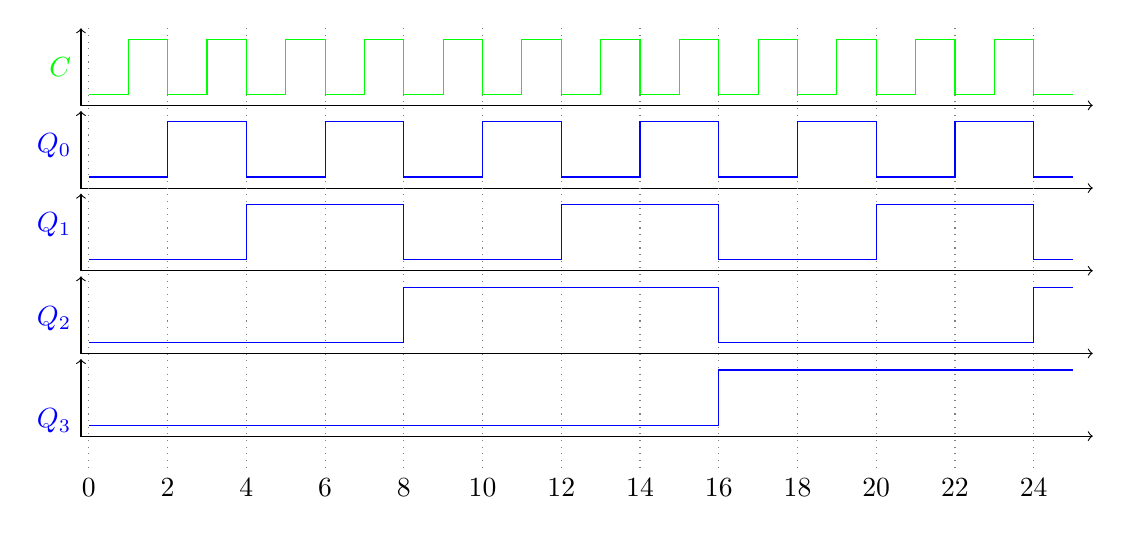
\begin{tikzpicture}[xscale=0.5, yscale=0.7]
        \draw[<->] (-0.2, 1.2) -- (-0.2, -0.2) -- (25.5, -0.2); 
        \draw[<->, yshift=-1.5cm] (-0.2, 1.2) -- (-0.2, -0.2) -- (25.5, -0.2); 
        \draw[<->, yshift=-3cm] (-0.2, 1.2) -- (-0.2, -0.2) -- (25.5, -0.2); 
        \draw[<->, yshift=-4.5cm] (-0.2, 1.2) -- (-0.2, -0.2) -- (25.5, -0.2); 
        \draw[<->, yshift=-6cm] (-0.2, 1.2) -- (-0.2, -0.2) -- (25.5, -0.2); 
        
        % Time labels and dotted lines for bottom graph only
        \foreach \x in {0, 2, 4, 6, 8, 10, 12, 14, 16, 18, 20, 22, 24} {
          \draw[dotted, gray] (\x, 1.2) -- (\x, -6.8);
          \node[below] at (\x, -6.8) {\x};
        }
        
        \node[green, left] at (-0.2, 0.5) {$C$}; 
        \node[blue, left, yshift=-1cm] at (-0.2, 0.5) {$Q_0$}; 
        \node[blue, left, yshift=-2cm] at (-0.2, 0.5) {$Q_1$}; 
        \node[blue, left, yshift=-3.2cm] at (-0.2, 0.5) {$Q_2$}; 
        \node[blue, left, yshift=-4.5cm] at (-0.2, 0.5) {$Q_3$}; 
        
        \draw[green] (0, 0) -- 
          (1, 0) -- (1, 1) -- (2, 1) -- (2, 0) -- 
          (3, 0) -- (3, 1) -- (4, 1) -- (4, 0) -- 
          (5, 0) -- (5, 1) -- (6, 1) -- (6, 0) -- 
          (7, 0) -- (7, 1) -- (8, 1) -- (8, 0) -- 
          (9, 0) -- (9, 1) -- (10, 1) -- (10, 0) -- 
          (11, 0) -- (11, 1) -- (12, 1) -- (12, 0) -- 
          (13, 0) -- (13, 1) -- (14, 1) -- (14, 0) -- 
          (15, 0) -- (15, 1) -- (16, 1) -- (16, 0) -- 
          (17, 0) -- (17, 1) -- (18, 1) -- (18, 0) -- 
          (19, 0) -- (19, 1) -- (20, 1) -- (20, 0) -- 
          (21, 0) -- (21, 1) -- (22, 1) -- (22, 0) -- 
          (23, 0) -- (23, 1) -- (24, 1) -- (24, 0) -- 
          (25, 0);
        \draw[blue, yshift=-1.5cm] (0, 0) -- 
          (2, 0) -- (2, 1) -- (4, 1) -- (4, 0) -- 
          (6, 0) -- (6, 1) -- (8, 1) -- (8, 0) -- 
          (10, 0) -- (10, 1) -- (12, 1) -- (12, 0) -- 
          (14, 0) -- (14, 1) -- (16, 1) -- (16, 0) -- 
          (18, 0) -- (18, 1) -- (20, 1) -- (20, 0) -- 
          (22, 0) -- (22, 1) -- (24, 1) -- (24, 0) -- 
          (25, 0); 
        \draw[blue, yshift=-3cm] (0, 0) -- 
          (4, 0) -- (4, 1) -- (8, 1) -- (8, 0) -- 
          (12, 0) -- (12, 1) -- (16, 1) -- (16, 0) -- 
          (20, 0) -- (20, 1) -- (24, 1) -- (24, 0) --
          (25, 0);
        \draw[blue, yshift=-4.5cm] (0, 0) -- 
          (8, 0) -- (8, 1) -- (16, 1) -- (16, 0) -- 
          (24, 0) -- (24, 1) -- (25, 1);
        \draw[blue, yshift=-6cm] (0, 0) -- 
          (16, 0) -- (16, 1) -- (25, 1);
      \end{tikzpicture}
      \caption{From $t = 0$ to $t = 1$, we have $Q = Q_3 Q_2 Q_1 Q_0 = 0000$. The next time period, we have $Q = 0001$, and so on. This is precisely a counter.}
    \end{figure}
  \end{example}

  This is extremely useful in almost every situation. First, we can now implement a program counter. Second, when multitasking in an operating system on a single core, we can have a scheduler that allows us to switch from one application to another. 

  If we connect the latches a bit differently, we can get a shift register, which allows us to do bit-shift operations. 

  \begin{definition}[Shift Registers]
    A \textbf{shift register} takes in a serial input and gives a serial output. It essentially does a bitshift. 
    \begin{align}
      Q(t + 1, \mathrm{in}) & = [ Q_3(t + 1), Q_2 (t + 1), Q_1 (t + 1), Q_0 (t + 1) ] = [ \mathrm{in}, Q_3 (t), Q_2 (t), Q_1 (t) ] \\ 
      \mathrm{out} & = Q_0 (t)
    \end{align} 

    \begin{figure}[H]
      \centering 
      \begin{tikzpicture}[circuit logic US, yscale=0.7, xscale=0.6]
        \foreach \x [count=\i from 0] in {0, 5, 10, 15} {
          \node[latch, align=center, scale=0.8] (latch) at (\x,0) {};
          \draw (latch.pin 1) -- ++(-1,0);
          \draw (latch.pin 3) -- ++(-0.5,0) node[left] {} -- ++ (0, -1) -- (-2, -1.95); 
          \draw (latch.pin 6) -- ++(1.3,0);
        }
        \node[left] (clk) at (-2.8, -1.95) {CLK};
        \draw (clk.east) -- (-1.8, -1.95);
        \node at (18.5, 1) {out}; 
        \node at (-2.8, 1) {in}; 
      \end{tikzpicture}
      \caption{4-bit register. Since $\overline{Q}$ is redundant we do not consider it as an output in our register. } 
    \end{figure}
  \end{definition}

  \begin{example}[4-Bit Shift Register] 
    Say that we start off with a buffer of $0000$, and we input in a $1$ every time interval. Then, with the clock, the flip-flops will make sure to update the shift register consistently. Note that $D_{\mathrm{in}}$ does not have to be perfectly initialized to $1$ at exactly the rising or falling edge. From our construction we have flexibility. 

    \begin{figure}[H]
      \centering 
      \begin{tikzpicture}[xscale=0.5, yscale=0.7]
        \draw[<->] (-0.2, 1.2) -- (-0.2, -0.2) -- (25.5, -0.2); 
        \draw[<->, yshift=-1.5cm] (-0.2, 1.2) -- (-0.2, -0.2) -- (25.5, -0.2); 
        \draw[<->, yshift=-3cm] (-0.2, 1.2) -- (-0.2, -0.2) -- (25.5, -0.2); 
        \draw[<->, yshift=-4.5cm] (-0.2, 1.2) -- (-0.2, -0.2) -- (25.5, -0.2); 
        \draw[<->, yshift=-6cm] (-0.2, 1.2) -- (-0.2, -0.2) -- (25.5, -0.2); 
        \draw[<->, yshift=-7.5cm] (-0.2, 1.2) -- (-0.2, -0.2) -- (25.5, -0.2); 
        
        % Time labels and dotted lines for bottom graph only
        \foreach \x in {0, 2, 4, 6, 8, 10, 12, 14, 16, 18, 20, 22, 24} {
          \draw[dotted, gray] (\x, 1.2) -- (\x, -8.3);
          \node[below] at (\x, -8.3) {\x};
        }
        
        \node[green, left] at (-0.2, 0.5) {$C$}; 
        \node[blue, left, yshift=-1cm] at (-0.2, 0.5) {$d_{\mathrm{in}}$}; 
        \node[red, left, yshift=-2cm] at (-0.2, 0.5) {$Q_0$}; 
        \node[red, left, yshift=-3.2cm] at (-0.2, 0.5) {$Q_1$}; 
        \node[red, left, yshift=-4.5cm] at (-0.2, 0.5) {$Q_2$}; 
        \node[red, left, yshift=-6cm] at (-0.2, 0.5) {$Q_3$}; 
        
        \draw[green] (0, 0) -- 
          (2, 0) -- (2, 1) -- (4, 1) -- (4, 0) -- 
          (6, 0) -- (6, 1) -- (8, 1) -- (8, 0) -- 
          (10, 0) -- (10, 1) -- (12, 1) -- (12, 0) -- 
          (14, 0) -- (14, 1) -- (16, 1) -- (16, 0) -- 
          (18, 0) -- (18, 1) -- (20, 1) -- (20, 0) -- 
          (22, 0) -- (22, 1) -- (24, 1) -- (24, 0) -- 
          (25, 0); 
        \draw[blue, yshift=-1.5cm] (0, 0) -- (2.4, 0) -- (2.4, 1) -- (25, 1);
        \draw[red, yshift=-3cm] (0, 0) -- (4, 0) -- (4, 1) -- (25, 1);
        \draw[red, yshift=-4.5cm] (0, 0) -- (8, 0) -- (8, 1) -- (25, 1);
        \draw[red, yshift=-6cm] (0, 0) -- (12, 0) -- (12, 1) -- (25, 1);
        \draw[red, yshift=-7.5cm] (0, 0) -- (16, 0) -- (16, 1) -- (25, 1);
      \end{tikzpicture}
      \caption{From $t = 0$ to $t = 4$, we have $Q = 0000$. From $t = 4$ to $t = 8$, we have $Q = 1000$. From $t = 8$ to $t = 12$, we have $Q = 1100$. From $t = 12$ to $t = 16$, we have $Q = 1110$. From $t = 16$ to $t = 20$, we have $Q = 1111$.}
    \end{figure}
  \end{example}

